\documentclass[a4paper,11pt]{book}
%\documentclass[a4paper,twoside,11pt,titlepage]{book}
\usepackage{listings}
\usepackage[utf8]{inputenc}
\usepackage[spanish]{babel}

\usepackage{float}
\usepackage{csquotes}

\usepackage{textcomp}

\usepackage{caption}
\usepackage{subcaption}


% Euro
\usepackage{eurosym}
\usepackage{multirow}

\usepackage{array}

% Matemáticas y algoritmos
\usepackage{amsmath}
\usepackage{amsfonts}
\usepackage[linesnumbered,ruled,vlined]{algorithm2e}

% Comandos matemáticos
\DeclareMathOperator*{\argmin}{arg\,min}

\usepackage[dvipsnames]{xcolor}

% nonl command
\let\oldnl\nl
\newcommand{\nonl}{\renewcommand{\nl}{\let\nl\oldnl}}

%\usepackage[style=list, number=none]{glossary} %
%\usepackage{titlesec}
%\usepackage{pailatino}

\decimalpoint
\usepackage{dcolumn}
\newcolumntype{.}{D{.}{\esperiod}{-1}}
\makeatletter
\addto\shorthandsspanish{\let\esperiod\es@period@code}
\makeatother


%\usepackage[chapter]{algorithm}
\RequirePackage{verbatim}
%\RequirePackage[Glenn]{fncychap}
\usepackage{fancyhdr}
\usepackage{graphicx}
\usepackage{afterpage}

\usepackage{longtable}

\usepackage[pdfborder={000}]{hyperref} %referencia

% ********************************************************************
% Re-usable information
% ********************************************************************
\newcommand{\myTitle}{Desarrollo de modelos de Machine Learning aplicando MLOps\xspace}
\newcommand{\myDegree}{Grado en Ingeniería Informática\xspace}
\newcommand{\myName}{Manuel Jesús Núñez Ruiz (alumno)\xspace}
\newcommand{\myProf}{Alberto Guillén Perales(tutor)\xspace}
%\newcommand{\mySupervisor}{Put name here\xspace}
\newcommand{\myFaculty}{Escuela Técnica Superior de Ingenierías Informática y de
Telecomunicación\xspace}
\newcommand{\myFacultyShort}{E.T.S. de Ingenierías Informática y de
Telecomunicación\xspace}
\newcommand{\myDepartment}{Departamento de Arquitectura y Tecnología de Computadores\xspace}
\newcommand{\myUni}{\protect{Universidad de Granada}\xspace}
\newcommand{\myLocation}{Granada\xspace}
\newcommand{\myTime}{\today\xspace}
\newcommand{\myVersion}{Version 0.1\xspace}


\hypersetup{
pdfauthor = {\myName manueljesusnunezruiz@gmail.com},
pdftitle = {\myTitle},
pdfsubject = {},
pdfkeywords = {palabra_clave1, palabra_clave2, palabra_clave3, ...},
pdfcreator = {pdflatex},
pdfproducer = {pdflatex}
}

%\hyphenation{}


%\usepackage{doxygen/doxygen}
%\usepackage{pdfpages}
\usepackage{url}
\usepackage{colortbl,longtable}
\usepackage[stable]{footmisc}
\usepackage{index}

%\makeindex
%\usepackage[style=long, cols=2,border=plain,toc=true,number=none]{glossary}
% \makeglossary

% Definición de comandos que me son tiles:
%\renewcommand{\indexname}{Índice alfabético}
%\renewcommand{\glossaryname}{Glosario}

\pagestyle{fancy}
\fancyhf{}
\fancyhead[LO]{\leftmark}
\fancyhead[RE]{\rightmark}
\fancyhead[RO,LE]{\textbf{\thepage}}
\renewcommand{\chaptermark}[1]{\markboth{\textbf{#1}}{}}
\renewcommand{\sectionmark}[1]{\markright{\textbf{\thesection. #1}}}

\setlength{\headheight}{1.5\headheight}

\newcommand{\HRule}{\rule{\linewidth}{0.5mm}}
%Definimos los tipos teorema, ejemplo y definición podremos usar estos tipos
%simplemente poniendo \begin{teorema} \end{teorema} ...
\newtheorem{teorema}{Teorema}[chapter]
\newtheorem{ejemplo}{Ejemplo}[chapter]
\newtheorem{definicion}{Definición}[chapter]

\definecolor{gray97}{gray}{.97}
\definecolor{gray75}{gray}{.75}
\definecolor{gray45}{gray}{.45}
\definecolor{gray30}{gray}{.94}

\lstset{ frame=Ltb,
     framerule=0.5pt,
     aboveskip=0.5cm,
     framextopmargin=3pt,
     framexbottommargin=3pt,
     framexleftmargin=0.1cm,
     framesep=0pt,
     rulesep=.4pt,
     backgroundcolor=\color{gray97},
     rulesepcolor=\color{black},
     %
     stringstyle=\ttfamily,
     showstringspaces = false,
     basicstyle=\scriptsize\ttfamily,
     commentstyle=\color{gray45},
     keywordstyle=\bfseries,
     %
     numbers=left,
     numbersep=6pt,
     numberstyle=\tiny,
     numberfirstline = false,
     breaklines=true,
   }
 
% minimizar fragmentado de listados
\lstnewenvironment{listing}[1][]
   {\lstset{#1}\pagebreak[0]}{\pagebreak[0]}

\lstdefinestyle{CodigoC}
   {
	basicstyle=\scriptsize,
	frame=single,
	language=C,
	numbers=left
   }
\lstdefinestyle{CodigoC++}
   {
	basicstyle=\small,
	frame=single,
	backgroundcolor=\color{gray30},
	language=C++,
	numbers=left
   }

 
\lstdefinestyle{Consola}
   {basicstyle=\scriptsize\bf\ttfamily,
    backgroundcolor=\color{gray30},
    frame=single,
    numbers=none
   }
   
\lstdefinelanguage{docker}{
  keywords={FROM, RUN, COPY, ADD, ENTRYPOINT, CMD,  ENV, ARG, WORKDIR, EXPOSE, LABEL, USER, VOLUME, STOPSIGNAL, ONBUILD, MAINTAINER},
  keywordstyle=\color{blue}\bfseries,
  identifierstyle=\color{black},
  sensitive=false,
  comment=[l]{\#},
  commentstyle=\color{Emerald}\ttfamily,
  stringstyle=\color{red}\ttfamily,
  morestring=[b]',
  morestring=[b]"
}


\newcommand{\bigrule}{\titlerule[0.5mm]}


%Para conseguir que en las páginas en blanco no ponga cabecerass
\makeatletter
\def\clearpage{%
  \ifvmode
    \ifnum \@dbltopnum =\m@ne
      \ifdim \pagetotal <\topskip
        \hbox{}
      \fi
    \fi
  \fi
  \newpage
  \thispagestyle{empty}
  \write\m@ne{}
  \vbox{}
  \penalty -\@Mi
}
\makeatother

\usepackage{footnote}

\usepackage{pdfpages}
\begin{document}

\renewcommand{\tablename}{Tabla}

\begin{titlepage}
 
 
\newlength{\centeroffset}
\setlength{\centeroffset}{-0.5\oddsidemargin}
\addtolength{\centeroffset}{0.5\evensidemargin}
\thispagestyle{empty}

\noindent\hspace*{\centeroffset}\begin{minipage}{\textwidth}

\centering

\includegraphics[width=0.9\textwidth]{imagenes/logo_ugr.jpg}\\[1.4cm]

\textsc{ \Large TRABAJO FIN DE GRADO\\[0.2cm]}
\textsc{ INGENIERÍA INFORMÁTICA}\\[1cm]
% Upper part of the page
% 
% Title
{\Huge\bfseries Desarrollo de modelos de Machine Learning\\
}
\noindent\rule[-1ex]{\textwidth}{3pt}\\[3.5ex]
{\large\bfseries Aplicando metodologías ágiles y las mejores prácticas}
\end{minipage}

\vspace{2.5cm}
\noindent\hspace*{\centeroffset}\begin{minipage}{\textwidth}
\centering

\textbf{Autor}\\ {Manuel Jesús Núñez Ruiz (alumno)}\\[2.5ex]
\textbf{Directores}\\
{Alberto Guillén Perales (tutor)}\\[2cm]

\includegraphics[width=0.3\textwidth]{imagenes/etsiit_logo.png}\\[0.1cm]
\textsc{Escuela Técnica Superior de Ingenierías Informática y de Telecomunicación}\\
\textsc{---}\\
Granada, Julio de 2021
\end{minipage}
%\addtolength{\textwidth}{\centeroffset}
%\vspace{\stretch{2}}
\end{titlepage}



%\chapter*{}
%\thispagestyle{empty}
%\cleardoublepage

%\thispagestyle{empty}

\cleardoublepage
\thispagestyle{empty}

\begin{center}
{\large\bfseries Título del Proyecto: Subtítulo del proyecto}\\
\end{center}
\begin{center}
Nombre Apellido1 Apellido2 (alumno)\\
\end{center}

%\vspace{0.7cm}
\noindent{\textbf{Palabras clave}: palabra\_clave1, palabra\_clave2, palabra\_clave3, ......}\\

\vspace{0.7cm}
\noindent{\textbf{Resumen}}\\

Poner aquí el resumen.
%\cleardoublepage
\newpage


\thispagestyle{empty}


\begin{center}
{\large\bfseries Project Title: Project Subtitle}\\
\end{center}
\begin{center}
First name, Family name (student)\\
\end{center}

%\vspace{0.7cm}
\noindent{\textbf{Keywords}: Keyword1, Keyword2, Keyword3, ....}\\

\vspace{0.7cm}
\noindent{\textbf{Abstract}}\\

Write here the abstract in English.

\chapter*{}
\thispagestyle{empty}

\noindent\rule[-1ex]{\textwidth}{2pt}\\[4.5ex]

Yo, \textbf{Manuel Jesús Núñez Ruiz}, alumno de la titulación TITULACIÓN de la \textbf{Escuela Técnica Superior
de Ingenierías Informática y de Telecomunicación de la Universidad de Granada}, con DNI 31027610N, autorizo la
ubicación de la siguiente copia de mi Trabajo Fin de Grado en la biblioteca del centro para que pueda ser
consultada por las personas que lo deseen.

\vspace{6cm}

\noindent Fdo: Manuel Jesús Núñez Ruiz

\vspace{2cm}

\begin{flushright}
Granada a X de Junio de 2021.
\end{flushright}


\chapter*{}
\thispagestyle{empty}

\noindent\rule[-1ex]{\textwidth}{2pt}\\[4.5ex]

D. \textbf{Alberto Guillén Perales (tutor)}, Profesor del Área de XXXX del Departamento Arquitectura y Tecnología de Computadores de la Universidad de Granada.



\vspace{0.5cm}

\textbf{Informan:}

\vspace{0.5cm}

Que el presente trabajo, titulado \textit{\textbf{Desarrollo de modelos de Machine Learning, Aplicando metodologías ágiles y las mejores prácticas}},
ha sido realizado bajo su supervisión por \textbf{Manuel Jesús Núñez Ruiz (alumno)}, y autorizamos la defensa de dicho trabajo ante el tribunal
que corresponda.

\vspace{0.5cm}

Y para que conste, expiden y firman el presente informe en Granada a X de Junio de 2021.

\vspace{1cm}

\textbf{El director:}

\vspace{5cm}

\noindent \textbf{Alberto Guillén Perales (tutor)}

\chapter*{Agradecimientos}
\thispagestyle{empty}

       \vspace{1cm}


Poner aquí agradecimientos...


\frontmatter
\tableofcontents
\listoffigures
\listoftables
%
\mainmatter
\setlength{\parskip}{5pt}

\chapter{Objetivos}

El objetivo general del proyecto es enfrentarse a un problema de Machine Learning real con una metodología ágil para producir y validar modelos predictivos e intentar obtener los mejores resultados posibles. De forma más específica, los objetivos serían los siguientes:

\begin{itemize}
	\item Llevar un control sobre los experimentos realizados así como de los artefactos generados con cada experimento.
	\item Obtener los mejores resultados posibles mediante el uso de los hiperparámetros óptimos en el entrenamiento de cada modelo.
	\item Controlar la validación de los modelos, es decir, que las entradas y las salidas de los mismos sea la esperada y que se optimicen correctamente.
	\item Despliegue de modelos de forma ágil, sin que el desarrollador tenga que gastar mucho tiempo en ello y pueda concentrarse en escribir/mejorar el código.
	\item Todo el código de este proyecto será liberado para que cualquier persona pueda consultarlo con fines académicos y/o colaborar mediante algún cambio o añadiendo alguna \textit{feature}. Obviamente tendrá su licencia para evitar plagios o algún otro uso indebido.
	\item Por último y no menos importante, este trabajo y sus resultados deben ser completamente reproducibles. Es decir, que puedan ser ejecutados en otro computador distinto con facilidad y que se obtengan los mismos resultados.
\end{itemize}

\chapter{Introducción}

\section{¿Qué es DevOps?}

\enquote{El término \textit{DevOps}, que es una combinación de los términos ingleses \textit{development} (desarrollo) y \textit{operations} (operaciones), designa la unión de personas, procesos y tecnología para ofrecer valor a los clientes de forma constante} \cite{devops}. Gracias a esta práctica y a sus herramientas, los roles que trabajan en el desarrollo del software pueden trabajar juntos para producir productos mejores y más confiables, además de hacer que mejore el rendimiento de los equipos y creen productos de calidad en menos tiempo.

\subsection{Prácticas DevOps}

La mayoría de las prácticas de \textit{DevOps} están diseñadas para agilizar, automatizar y mejorar las fases del desarrollo del software, reduciendo el riesgo de errores humanos y mejorando la velocidad.

\begin{itemize}
	\item \textbf{Integración y Despliegue Continuos (CI/CD).} Mediante la práctica de Integración Continua, cada vez que se fusionan los cambios en la rama de código principal (cada vez que se realiza un \enquote{commit}), se realizan pruebas automáticas para garantizar la estabilidad de la rama principal \cite{devops}.\\
	
	El Despliegue Continuo es la automatización de la puesta en producción de los nuevos cambios y también se ejecuta al fusionar nuevos cambios en la rama principal. De esta forma, es mucho más rápido el proceso del despliegue al no tener que hacerlo manualmente y nos permite realizar implementaciones más frecuentes \cite{devops}.
	
	\item \textbf{Control de versiones.} \enquote{Es la práctica que nos permite administrar el código por versiones y del historial de cambios para facilitar la revisión y la recuperación del código} \cite{devops}. El sistema que nos brinda esta utilidad es \textit{git} y el código suele estar publicado en un repositorio remoto (que puede ser privado o público) usando este mismo sistema para que todo el equipo tenga acceso al control de versiones.
	
	\item \textbf{Infraestructura como Código.} \enquote{Permite definir las topologías y los recusos de un modo descriptivo que permite a los equipos administrar esos recursos igual que lo harían con el código} \cite{devops}. Además, al estar definida como código, se puede administrar sus versiones con el sistema de control de versiones. En adición, hace que la creación de la infraestructura sea repetible y ayuda a automatizar el Despliegue continuo.
	
	\item \textbf{Administración de configuración.} Podemos usarla junto con la Infraestructura como Código para automatizar la definición y configuración de sistemas \cite{devops}. Es muy común guardar la configuración de un sistema en un fichero con un formato determinado (si no contiene información confidencial como contraseñas), como variable de entorno en una única máquina o usar un mecanismo de configuración distribuida si utilizamos un cluster (como por ejemplo etcd \cite{etcd}).
	
	\item \textbf{Monitorización.} Consiste en visualizar en tiempo real el rendimiento y el estado de la pila de aplicaciones, desde la infraestructura subyacente hasta el software de niveles superiores con el fin de mitigar los errores producidos durante la ejecución de la misma o ver si es necesario escalarla \cite{devops}.
\end{itemize}

\subsection{DevOps y contenedores}

\enquote{Los contenedores linux son una tecnología que nos permite empaquetar y aislar aplicaciones junto con su entorno de ejecución (todos los archivos necesarios para que funcione)} \cite{containers}. Esto nos permite que la aplicación se pueda ejecutar en cualquier máquina/arquitectura que ejecute Linux sin problemas (solo se tiene que tener instalado algún \textit{container engine}) y con mucha facilidad, pues los contenedores son portables. Para esto, existe en internet un gran número de repositorios de contenedores, que  nos permite subirlos de manera gratuita y descargarlo en otra máquina. Gracias a esta tecnología, podemos facilitar mucho el flujo de CI/CD al poder ejecutar la aplicación y sus tests en un contenedor.\newline

\section{Motivación para usar MLOps}

Hoy en día, en los proyectos de Machine Learning, el código dedicado a definir los modelos predictivos representa una fracción muy pequeña comparada con otros componentes del flujo de trabajo. Para poder operar con modelos, los científicos de datos deben de trabajar junto con otras personas que se dedican a eso mismo, operaciones (encargados de desplegar, testear el sistema, aprovisionar la infraestructura necesaria, etc). Esto representa un desafío en la organización en términos de comunicación, colaboración y coordinación. El objetivo de MLOps es enfrentarse a dicho desafío estableciendo buenas prácticas para el desarrollo. Además, nos aporta de la velocidad y agilidad necesaria en el mundo digital actual.

\begin{figure}[h]
	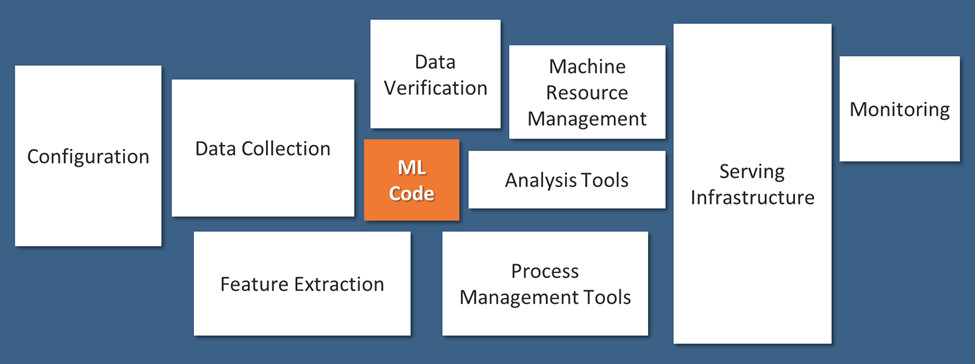
\includegraphics[scale=1]{imagenes/01_Introduccion/mlcodefraction.jpg}
	\centering
	\caption{Como se muestra en la figura, la fracción de código en los sistemas de ML reales es bastante pequeña. En cambio la fracción de infraestructura es mucho mayor \cite{NIPS2015_86df7dcf}.}
\end{figure}

En este caso, adoptar las mejores prácticas de \textbf{DevOps} podría ser posible, pues el Machine Learning tiene mucho en común con la ingeniería del software. La diferencia es que en Machine Learning hay que llevar un registro de modelos y sus hiperparámetros, con el fin de que el experimento se pueda replicar con la mayor facilidad en otro sistema (esto recibe el nombre de reproducibilidad) \cite{whymlops}.\newline

En DevOps y MLOps se debe de usar un sistema de control de versiones (git) para poder gestionar los cambios en el código. Adicionalmente, en MLOps necesitamos versionar los modelos y sus hiperparámetros, pero gracias a la herramienta DVC (su uso está explicado en un capítulo posterior) esto ya no es problema. Además de todo lo anterior, el código debe de estar subido a un repositorio remoto compartido (como puede ser GitHub, GitLab, Bitbucket, etc) para poder trabajar cómodamente en equipo. En este repositorio debemos tener el control de que en cada cambio incremental todo lo anterior y lo nuevo siga funcionando, por lo tanto es necesario el uso de lo que se llama Integración Continua. Este proceso de Integración Continua lo que hace es ejecutar los tests que hemos escrito sobre el código implementado para comprobar que efectivamente funciona como esperábamos. En cuanto a MLOps, también es necesario testear que los modelos se comporten como esperamos. Esto nos permite desarrollar software de mayor calidad y con una altísima frecuencia de releases.\newline

Además de lo anterior, también se puede configurar un Despliegue Continuo, así si nuestro código pasa con éxito los tests de Integración Continua, podriamos desplegarlo en cuestión de segundos o unos pocos minutos mediante otras herramientas/plataformas que nos permitan acelerar dicho despliegue usando Infraestructura como Código. Para poder integrar la Integración Continua y el Despliegue Continuo (a partir de ahora lo llamaremos CI/CD) nos hace falta una plataforma en la nube que nos lo permita. Todo esto está desarrollado en los próximos capítulos de este documento.

\section{Descripción del problema}

La Tierra está siendo \enquote{bombardeada} constantemente con rayos cósmicos que provienen, como su nombre indica, del universo. Estos rayos se componen de partículas que viajan a la velocidad de la luz, que al entrar en contacto con la atmósfera producen una cascada atmosférica extensa. Dicha cascada emite una luz debido a la radiación gamma llamada \enquote{Luz de Cherenkov}. A la misma vez, el rayo cósmico se fragmenta formando hadrones. Es decir, estos rayos se descomponen en una componente hadrónica y otra componente electromagnética.\newline

\enquote{La detección de de rayos gamma de muy alta energía es esencial para investigar las fuentes de la radiación entrante producida por alguno de los fenómenos más extremos que suceden en el universo, por ejemplo estrellas de neutrones y agujeros negros supermasivos} \cite{gonzalez2021tackling}.

\begin{figure}[H]
	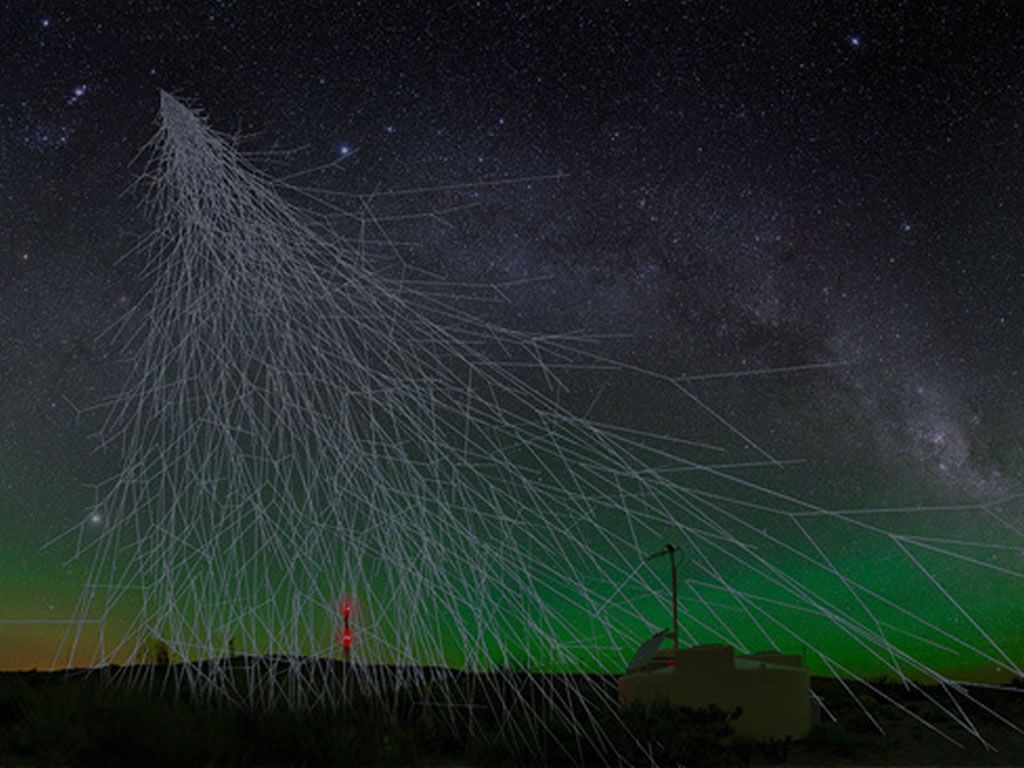
\includegraphics[scale=.3]{imagenes/01_Introduccion/EAS.jpg}
	\centering
	\label{fig:wcd}
	\caption{Así sería una Cascada Atmosférica Extensa incidiendo sobre un Water Cherenkov Detector (WCD). Fuente: \href{https://revolucion.news/cienciario.mx/los-rayos-cosmicos-de-muy-alta-energia-vienen-de-fuera-de-la-via-lactea/}{revolucion.news}.}
\end{figure}

Para poder capturar información sobre dichos rayos cósmicos, se usan WCD (se puede ver la imagen de uno en la Figura \ref{fig:wcd}) que son tanques de agua ultrapura que contienen fotomultiplicadores distribuidos simétricamente dentro del tanque que se utilizan para captar la señal del rayo que incide sobre el mismo. En función de la profundidad del agua del WCD, se emitirá más luz o menos, siendo directamente proporcionales.\newline

El problema que se pretende solucionar en este proyecto, es diseñar un modelo que sea capaz de diferenciar un rayo que sea solo radiación gamma electromagnética de uno que tenga una partícula denominada \enquote{muón}. Esta partícula se genera por la interacción a alta energía de los hadrones y nos permiten discriminar bastante bien entre la radiación gamma y los hadrones \cite{gonzalez2021tackling}.

\begin{figure}[H]
	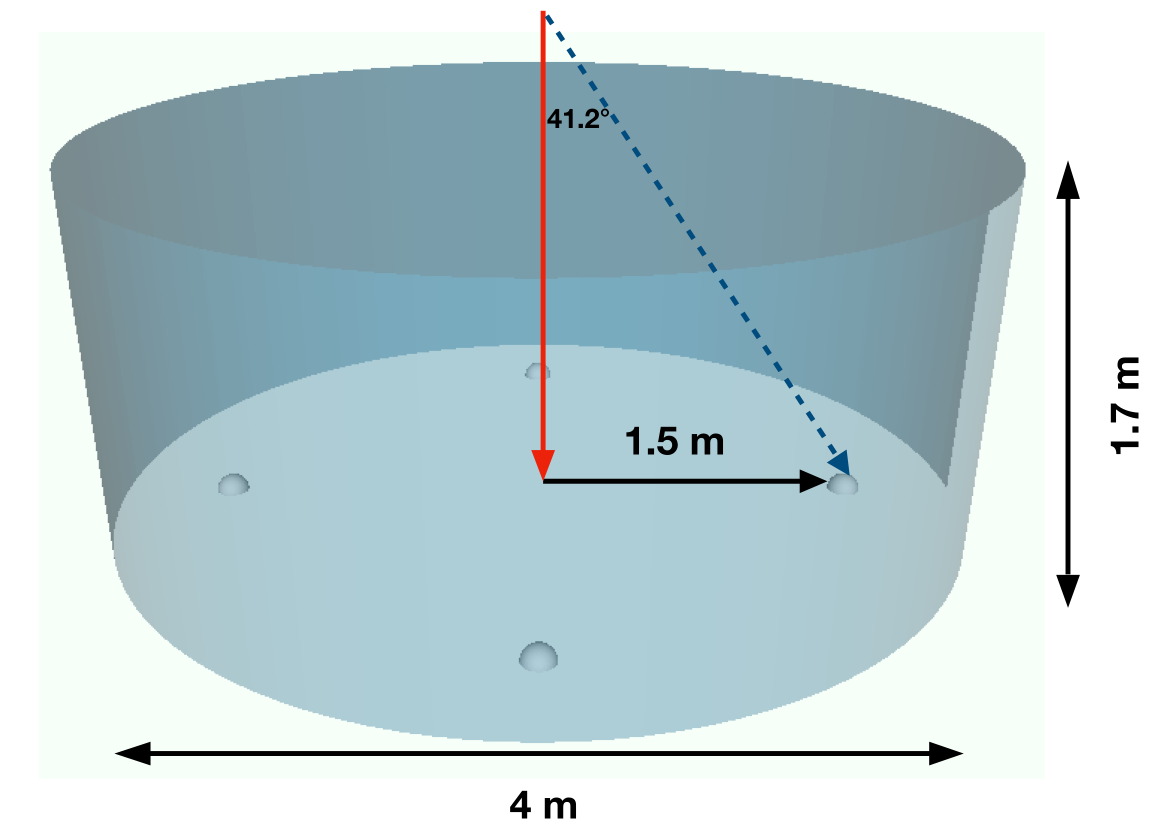
\includegraphics[scale=.1]{imagenes/01_Introduccion/wcd.png}
	\centering
	\caption{Diseño de un WCD \cite{gonzalez2021tackling}.}
\end{figure}


\chapter{Estado del arte}

\section{Ingeniería del Software}

En esta sección voy a describir las herramientas que se usarán en este proyecto así como la justificación del uso de cada una. Todas están enfocadas para lograr las mejores prácticas de la metodología DevOps.

\subsection{Lenguaje elegido}

El lenguaje que he elegido para la realización de este proyecto ha sido Python, por ser muy fácil de aprender y además tiene un gran número de librerías para ciencia de datos.

\subsection{Gestor de dependencias}

El gestor de dependencias es una herramienta muy útil hoy en día para poder manejar las dependencias de una aplicación o un proyecto de forma sencilla, usando las órdenes del mismo. Además nos permite instalar todas las librerías usando únicamente una orden. Esto claramente ayuda a mantener la reproducibilidad de la aplicación ya que facilita bastante la ejecución de la misma aplicación en otra máquina (como por ejemplo en el entorno de Integración continua, en la máquina de entrenamiento de modelos o en la que desplegaremos un microservicio). En Python, los dos principales gestores de dependencias son \enquote{Pipenv} y \enquote{Poetry}.Ambas herramientas gestionan por debajo un entorno virtual aislado que contiene las dependencias instaladas.

\subsubsection*{Pipenv}

Pipenv se define como una herramienta que apunta a traer todo lo mejor del mundo del empaquetado al mundo Python \cite{pipenv}. Usa un fichero con sintaxis TOML para registrar las dependencias cuyo nombre es Pipfile.

\subsubsection*{Poetry}

Poetry es una herramienta cuya popularidad está creciendo un montón actualmente en la comunidad de Python. Es utilizada únicamente para manejar las dependencias de cualquier proyecto de forma muy sencilla. Además, cuenta con una documentación muy buena y clara \cite{poetry}.

\subsubsection*{Comparación de ambas herramientas}

Para comparar ambas herramientas para el manejo de dependencias, voy a utilizar el tiempo que tardan en instalar las librerías usando el fichero \textit{lock}. Las librerías que he usado como dependencias han sido \textit{PyTorch} y \textit{FastAPI} y de dependencias de desarrollo \textit{pylint} y \textit{pytest}. En la siguiente tabla se pueden ver los resultados:

\begin{table}[h]
\begin{tabular}{|c|c|c|}
\hline
                     & \textbf{Pipenv} & \textbf{Poetry} \\ \hline
\textbf{Ejecución 1} & 31,938          & 22,009          \\ \hline
\textbf{Ejecución 2} & 38,528          & 23,068          \\ \hline
\textbf{Ejecución 3} & 33,63           & 23,111          \\ \hline
\textbf{Ejecución 4} & 35,452          & 21,407          \\ \hline
\textbf{Ejecución 5} & 33,406          & 20,901          \\ \hline
\textbf{Media}       & 34,59           & 22,10           \\ \hline
\end{tabular}
\centering
\caption{Tiempo (medido en segundos) que tarda cada herramienta en instalar las dependencias anteriores.}
\label{tab:poetryvspipenv}
\end{table}

Como se puede ver en el Cuadro \ref{tab:poetryvspipenv}, Poetry es siempre más rápido que Pipenv, por lo tanto usaré Poetry para manejar las dependencias del proyecto. Además me gustaría añadir que en el momento del testeo, intenté instalar la librería \textit{black}, pero Pipenv me dió problemas, cosa que con Poetry no pasó. He hecho el test de tiempo debido a que necesito que se instalen las dependencias lo más rápido posible para que la Integración Continua dure lo menos posible en ejecutarse y para que se despliegue rápido la aplicación, ya que la instalación de dependencias es casi siempre lo que más tarda.

\subsection{Gestor de tareas}

Para seguir ayudando con la reproducibilidad del proyecto, necesitamos un gestor que contenga las órdenes necesarias para testear o arrancar la aplicación o lanzar el entrenamiento de modelos. Esto nos permite que nuestro proyecto se pueda ejecutar en otra máquina de forma sencilla, ejecutando una sola orden que ya lo hace todo por nosotros. Poetry no trae por defecto ningún gestor de tareas, al contrario que Pipenv que sí lo trae. Pero por suerte, existe una herramienta que nos añade un task manager en Poetry llamada \textit{Poethepoet}. Esta herramienta nos permite lanzar una tarea tan solo escribiendo \textit{poe $<taskname>$} \cite{poethepoet}.

\subsection{Plataforma de CI/CD}

La finalidad de esta plataforma es ejecutar los tests y realizar el despliegue cada vez que se produzca un incorporación de código al repositorio de GitHub. Se usará para controlar los cambios en el código. En la CI, lo que hace es ejecutar los tests para comprobar que todo funcione bien. Si la CI tiene éxito, los cambios se aprueban y se combinan en el repositorio compartido y se despliega la aplicación en la máquina destino. Esto sería así en DevOps, pero en MLOps tenemos que entrenar los modelos antes de desplegarlos, por lo cuál el workflow se hace un poco más complejo.

\begin{figure}[h]
	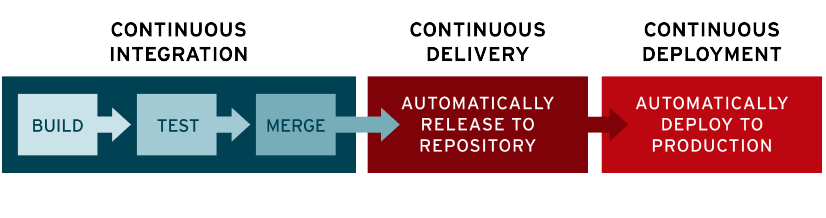
\includegraphics[scale=0.4]{imagenes/03_Estado_del_arte/ci-cd-flow.png}
	\centering
	\caption{Flujo de trabajo CI/CD. \cite{cicd}}
\end{figure}

Casi todas las plataformas de CI/CD tienen un plan de pago pero también tienen un plan gratuito. Mi criterio al seleccionar una plataforma de CI/CD concreta es gastar el menor dinero posible. Por ejemplo Travis, una plataforma que antes era gratuita y es muy rápida, otorgan ahora 10.000 créditos de los cuales, debido al uso que le di en una asignatura, solo me quedan 1650, por lo que esta plataforma queda descartada. En el caso de CircleCI, otorga 2.500 créditos gratis al mes, lo cual limitaría el número de subidas de código que puedo realizar en un mes y no me convence demasiado.\newline

Existen algunas plataformas gratuitas como por ejemplo Shippable, pero es demasiado lenta. GitHub Actions también es gratuita para repositorios públicos, como es el caso por lo que estaría interesante usarlo para comprobaciones básicas del repositorio, como por ejemplo comprobar la presencia de archivos importantes del mismo o comprobar la ortografía del README.\newline

Una plataforma a la que seguro le daré uso será Jenkins, tal vez una de las plataformas de CI/CD más populares escrita en Java. Esta plataforma es muy configurable y además dispone de un montón de plugins desarrollados por la comunidad que añaden un montón de utilidades. Para hacerlo funcionar, tenemos que instalarlo en un computador, por lo que sería necesario una instancia en alguna plataforma cloud para tenerlo disponible el mayor tiempo posible o incluso se podría ejecutar en una Raspberry Pi, lo único que necesitamos para que funcione es una Máquina Virtual Java. En mi caso tengo 150\$ en la plataforma AWSEducate, por lo que podría desplegar una instancia con Jenkins estando disponible el mayor tiempo posible sin problemas.\newline

Todas las plataformas anteriores disponen de un fichero de configuración que se almacena en el repositorio en el que hay que describir la secuencia de órdenes para poder ejecutar los tests o hacer el despliegue, además de especificar el contenedor en el que ese ejecuta, versiones del lenguaje, etc.

\subsection{Framework para MLOps}

Lo que necesito de un framework para MLOps es que registre los experimentos realizados (hiperparámetros usados y resultados obtenidos) y además nos facilite la reproducibilidad de los mismos, es decir, que se obtengan los mismos resultados independientemente de la máquina/entorno en el que se ejecuten.\newline

Existe un framework llamado SnapperML que facilita todo lo anterior. Permite almacenar los hiperparámetros de los modelos en formato YAML, además de tener un control de la estocasticidad (recoge información sobre la semilla utilizada para los diferentes generadores de números aleatorios). También permite el \textit{tracking} de experimentos usando \textit{MLFlow}, una herramienta que permite registrar métricas, hiperparámetros y artefactos y nos permite acceder a ellos a través de una interfaz web bastante intuitiva. Además de todo lo anterior, usa una librería llamada \textit{Optuna} para la optimización de hiperparámetros y \textit{Ray} para la ejecución en cluster \cite{snapperml}.\newline

Como se puede ver, este framework es todo lo que necesito para conseguir la reproducibilidad de los modelos de Machine Learning, pues la reproducibilidad del software ya está conseguida gracias a los gestores de dependencias y de tareas.

\subsection{Aprovisionamiento de Infraestructura Virtual}

Otro detalle que no se nos puede olvidar, es la reproducibilidad de la infraestructura para que la misma pueda ser creada y aprovisionada en otras cuentas de la misma plataforma cloud de forma rápida y fácil. ¿Para qué queremos aprovisionar una infraestructura? En este caso, es necesaria por ejemplo para aprovisionar una instancia de EC2 con \textit{Jenkins}.\newline

Para esto existen dos alternativas: \textit{Pulumi} \cite{pulumi} y \textit{Terraform} \cite{Terraform}. Ambas nos dejan describir la Infraestructura como Código (IaC), lo que nos facilita un montón la reproducibilidad. Las diferencias entre ambos son las siguientes:

\begin{itemize}
	\item \textbf{Lenguaje de programación}: \textit{Terraform} usa Hashicorp Configuration Language (HCL), un lenguaje propio declarativo para poder describir nuestra infraestructura. Con \textit{Pulumi}, se puede usar un lenguaje de programación de propósito general (\textit{TypeScript}, \textit{JavaScript}, \textit{Python}, \textit{Go} o \textit{C\#}). Usar un lenguaje de propósito general puede ser más cómodo que usar uno declarativo, pues por ejemplo nos permite usar estructuras condicionales si llega a ser necesario.
	\item \textbf{Documentación}: a día de hoy \textit{Terraform} tiene una documentación más completa que \textit{Pulumi}. Es por eso que a lo mejor también tiene una mayor comunidad que \textit{Pulumi}.
	\item \textbf{Modularidad}: \textit{Terraform} presenta una mejor modularidad que \textit{Pulumi}, esto es gracias a que presenta componentes que son perfectamente reusables.
\end{itemize}

En conclusión, ambas herramientas están muy bien diseñadas, cada una tiene sus pros y sus contras. No obstante, he decidido usar \textit{Terraform} para aprovisionar las máquinas necesarias para este proyecto debido a que tener una buena documentación es algo que debería ser esencial hoy en día para poder aprender a usar dicha herramienta sin problemas o consultarla cuando algo falle.

\subsection{Contenedores}

\enquote{Los contenedores linux son una tecnología que nos permite empaquetar y aislar aplicaciones junto con su entorno de ejecución (todos los archivos necesarios para que funcione)} \cite{containers}. Esto nos permite que la aplicación se pueda ejecutar en cualquier máquina/arquitectura que ejecute Linux sin problemas (solo se tiene que tener instalado algún \textit{container engine}) y con mucha facilidad, pues los contenedores son portables. Para esto, existe en internet un gran número de repositorios de contenedores, que  nos permite subirlos de manera gratuita y descargarlo en otra máquina.\newline

Además de los anterior, los contenedores no se ejecutan sobre un hipervisor que funcionan sobre el Sistema Operativo Host, como sí hacen las máquinas virtuales, sino que se ejecutan como un proceso más y comparten el Kernel. Esto hace que las imágenes de los contenedores sean ligeras y además no degrade el rendimiento de la aplicación al no necesitar una capa de abstracción sobre el Sistema Operativo Host.\newline

Otra gran característica de esta tecnología es que se puedan desarrollar nuevas actualizaciones del propio contenedor de forma fácil, pues utilizan por debajo un sistema de versionamiento.

\begin{figure}[H]
	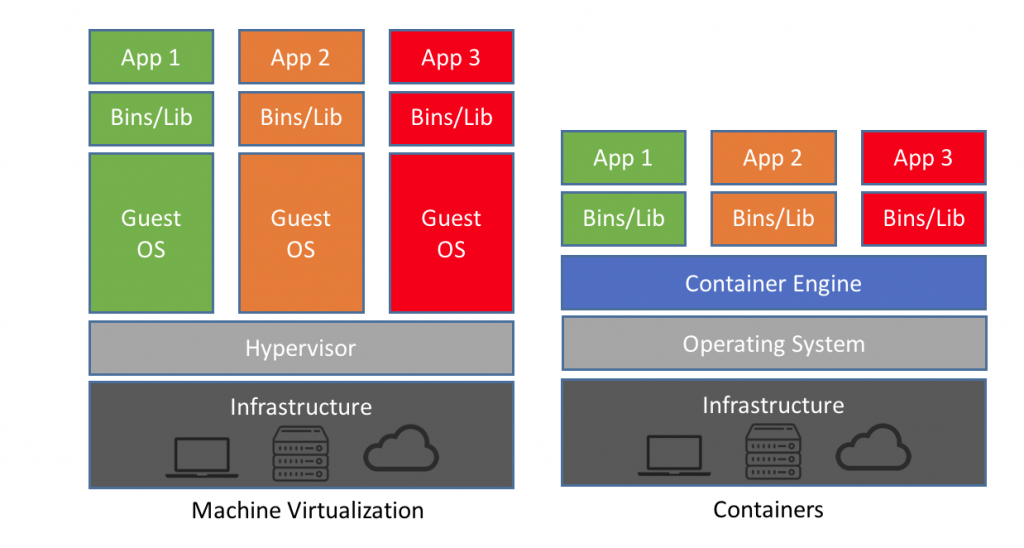
\includegraphics[scale=0.3]{imagenes/03_Estado_del_arte/containers.png}
	\centering
	\caption{Diferencia entre un contenedor y una Máquina Virtual.}
\end{figure}

Entre los \textit{container engines} más populares tenemos \textit{Docker} \cite{docker} y \textit{Podman} \cite{podman}. Recientemente, \textit{Docker} ha sido deprecado en \textit{Kubernetes} (una tecnología para orquestar contenedores ejecutándose en un cluster) debido a problemas de seguridad que presenta su diseño (usa un demonio para funcionar y ejecuta los contenedores con permisos root). \textit{Podman} arregla los problemas que presenta \textit{Docker}, pues no necesita de un demonio para ejecutarse y es \textit{rootless} por tanto es un \textit{engine} más seguro.

\section{Modelos de Machine Learning y Deep Learning}

En esta sección se describirán los modelos de Machine Learning o Deep Learning que se planean usar en los experimentos sobre el dataset.


\chapter{Planificación}

Para realizar este proyecto, lo he dividido en varias etapas. La primera etapa consta de definición del problema, búsqueda de objetivos e investigación del estado del arte (el cual ha sido abordado en los capítulo 1, 2 y 3 de este documento). La segunda etapa consistirá en un aprovisionamiento de la infraestructura necesaria para los tests del software o de los modelos predictivos. La tercera etapa consistirá en implementación y experimentación de los modelos predictivos usando uno o varios frameworks de Machine Learning o Deep Learning. Y por último, una cuarta etapa de implementación, despliegue y monitorización de un microservicio básico y la realización de los tests de infraestructura necesarios.\\

La metodología que usaré para llevar a cabo el proyecto será \textit{Kanban} \cite{kanban}. Esta metodología usa las llamadas \textit{Historias de Usuario} para reflejar los deseos de los clientes, las cuales tengo en \textit{GitHub} enunciadas en los \textit{issues} de este proyecto \cite{issues}. Además de lo anterior, en esta metodología se utiliza un tablero que nos permite visualizar el flujo del trabajo. En este tablero se encuentran las tareas necesarias en tres columnas distintas: \textit{To do} (aún no se ha empezado), \textit{In progress} (se está realizando ahora mismo) y \textit{Done} (finalizada).\\

Además de los anterior, \textit{GitHub} también nos permite agrupas las \textit{issues} en \textit{milestones}, cada milestone representará una etapa de este proyecto y haré uno especial para las Historias de Usuario y otro para documentación. Y si lo de antes es poco, también nos permite añadir un tablero \textit{kanban} al repositorio. En la Figura \ref{fig:kanban} se puede observar el que yo he realizado.\\

Podemos ver que \textit{GitHub} es una gran herramienta para el desarrollo de software que nos permite trabajar cómodamente de forma individual o en grupos.

\begin{figure}[H]
	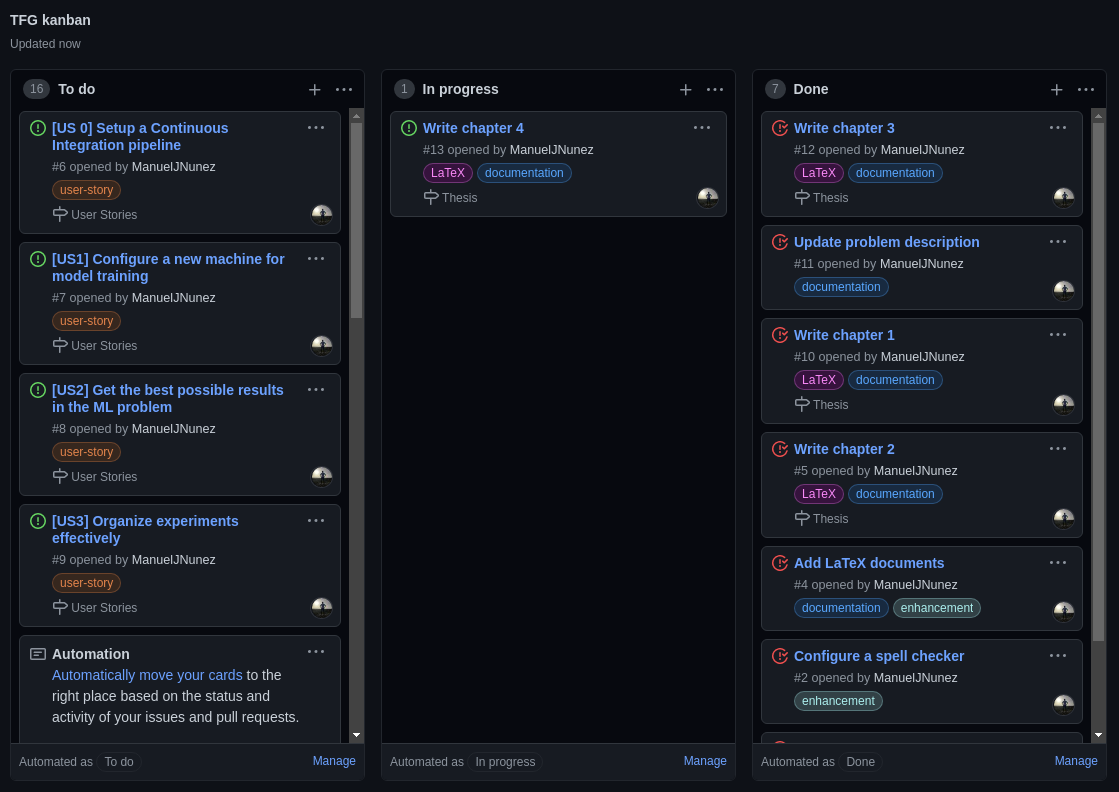
\includegraphics[scale=0.3]{imagenes/04_Planificacion/kanban.png}
	\centering
	\caption{Tablero \textit{kanban} en \textit{GitHub}. \cite{mykanban}}
	\label{fig:kanban}
\end{figure}


\chapter{Implementación}

\section{Modelos implementados}

Un aspecto importante a tener en cuenta sobre la implementación del código es que el desarrollo del código se ha llevado a cabo teniendo en cuenta la calidad del mismo. Además de eso, se han usado características avanzadas de Python como los \textit{type hints} para indicar en el código de que tipo son las variables requeridas por una función y el tipo de variable que devuelve.\newline

Otro aspecto importante que me gustaría recalcar es que todos los modelos han sido testeados usando \textit{Pytest}, lo que me ha permitido encontrar varios bugs antes de ponerme a usarlos.\\

\subsection{Neural Network Classifier}

Este modelo ha sido implementado para poder tener un número variable de capas y de neuronas con el de uasr el optimizador de hiperparámetros. Básicamente, el inicializador tiene como parámetros una lista de número enteros que representa el número de neuronas por cada capa, además de tener otro que representa el número de neuronas en la última capa. Utiliza una \textit{batch normalization} unidimensional y \textit{ReLU} como función de activación. En la última capa hace uso de \textit{Softmax} para calcular la probabilidad de pertenencia a alguna de las clases.\\

\subsection{Convolutional Autoencoder}\label{subsec:cae}

Este modelo fue explicado en la Subsección \ref{subsub:convautoencoder} y tiene los siguientes hiperparámetros:

\begin{itemize}
	\item El número de canales de salida de la primera convolución y el de las siguientes convoluciones se calculan como el número de canales de salida de la anterior multiplicado por dos.
	\item La profundidad del modelo, es decir, cuántas capas convolucionales tiene el \textit{encoder} y el \textit{decoder}.
	\item Tamaño del código del espacio latente.
	\item Número de canales de salida en la primera capa convolucional.
\end{itemize}

Al igual que el \textit{Varitional Autoencoder}, este modelo también hace uso de un \textit{Neural Network Classifier} para la clasificación del código del espacio latente.

\subsection{Convolutional Network Classifier}\label{subsec:convnet}

Este modelo está basado en \textit{LeNet-5} \cite{Lecun98gradient-basedlearning}, con una ligera modificación para poder probar algunas combinaciones en el optimizador de hiperparámetros. Esa modificación es que tiene un número de canales de salida para la convoluciones variable. Este modelo, al igual que los anteriores, usa un modelo de \textit{Neural Network Classifier} a la salida de la última capa de \textit{subsampling}.

\begin{figure}[H]
	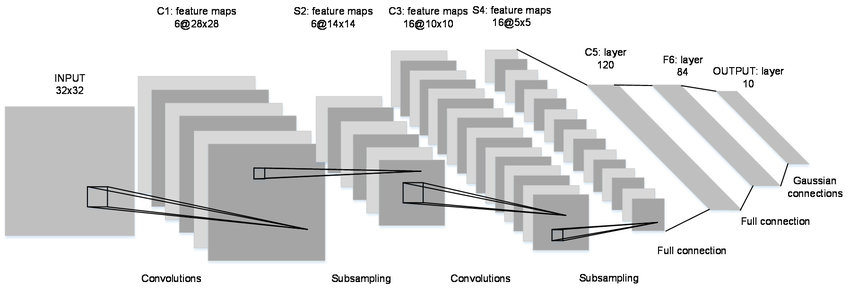
\includegraphics[scale=0.4]{imagenes/05_Implementacion/lenet5.png}
	\centering
	\caption{Estructura de \textit{LeNet-5}. \cite{Lecun98gradient-basedlearning}}
	\label{fig:convnet}
\end{figure}

\subsection{Residual Network Model}\label{subsec:resnetarch}
\label{subsec:resnet}

Para la simplificación del código de este modelo, he creado una clase que contiene las capas convolucionales necesarias para formar un \textit{ResNet block} (se pueden ver ejemplos de estos en la Figura \ref{fig:resnetblocks}). Como se ve en la Figura \ref{fig:resnet}, los \textit{Resnet Blocks} se agrupan en grupos que tienen en común un mismo número de canales en su input. En el primer \textit{ResBlock} de cada grupo, se divide entre dos la altura y la anchura de la imagen y se usa una convolución con tamaño de kernel 1x1 para poder hacer un \textit{downsample} y poder sumar las activaciones de entrada al \textit{ResBlock} con las de salida de la última convolución. Los hiperparámetros de este modelo son:

\begin{itemize}
	\item Número de canales con los que trabaja cada grupo de \textit{ResBlocks}.
	\item Número de \textit{ResBlocks} en cada grupo.
\end{itemize}

Al final de los grupos de \textit{ResBlocks}, uso una capa de \textit{Adaptative Average Pool} para dejar la salida en un vector de tamaño 512x1x1 y usar un \textit{Classifier Neural Network} para clasificar ese \textit{output}.

\begin{figure}[H]
	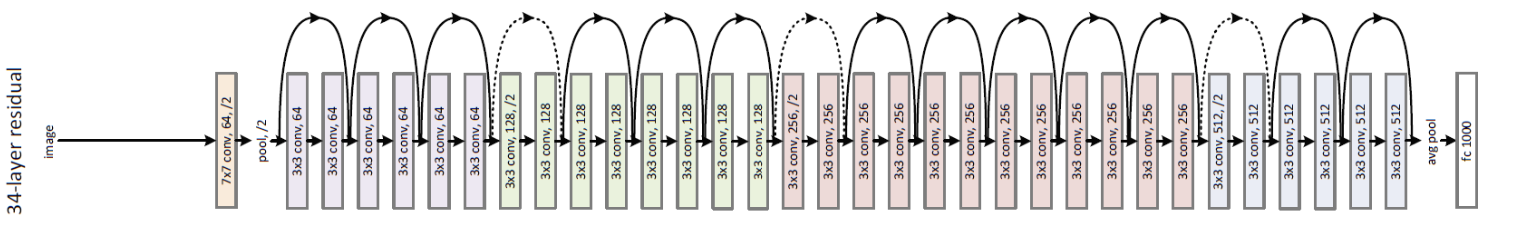
\includegraphics[width=1.\linewidth]{imagenes/05_Implementacion/resnet.png}
	\centering
	\caption{Ejemplo de \textit{ResNet}. \cite{DBLP:journals/corr/HeZRS15}}
	\label{fig:resnet}
\end{figure}

\subsection{Varitional Autoencoder}\label{subsec:vae}

Al igual que el \textit{Neural Network Classifier}, este modelo tiene un número variable de capas y de neuronas por capa. Tiene como parámetro una lista de enteros, que representa el tamaño de las capas del \textit{encoder} si la recorremos de principio a final y la del \textit{decoder} si la recorremos desde el final al principio (el autoencoder es simétrico). A parte, hace uso de una instancia del modelo \textit{Neural Network Classifier} para la clasificación del código latente del autoencoder. Un ejemplo gráfico de este autoencoder puede ser visto en la sección \ref{fig:classiferautoencoder}.\\

\section{Infraestructura Virtual y Metodología de uso}

En las próximas subsecciones se van a detallar las infraestructuras virtuales levantadas para llevar a cabo la realización de este proyecto y el uso que les he dado sin dejar atrás cómo se integran unas con otras.\\

Para este proyecto he diseñado dos infraestructuras diferentes:

\begin{itemize}
    \item \textbf{Infraestructura de test.} Como su propio nombre indica, se encarga de ejecutar los tests y además, de la evaluación del código fuente.
    \item \textbf{Infraestructura de entrenamiento.} Utilizada para entrenar modelos y almacenar los hiperparámetros y las métricas. Para el entrenamiento de los mismos se ha utilizado la GPU de mi portátil personal y las GPUs del clúster \textit{HPMOON}.
\end{itemize}

\subsection{Infraestructura de test}

\begin{figure}[H]
	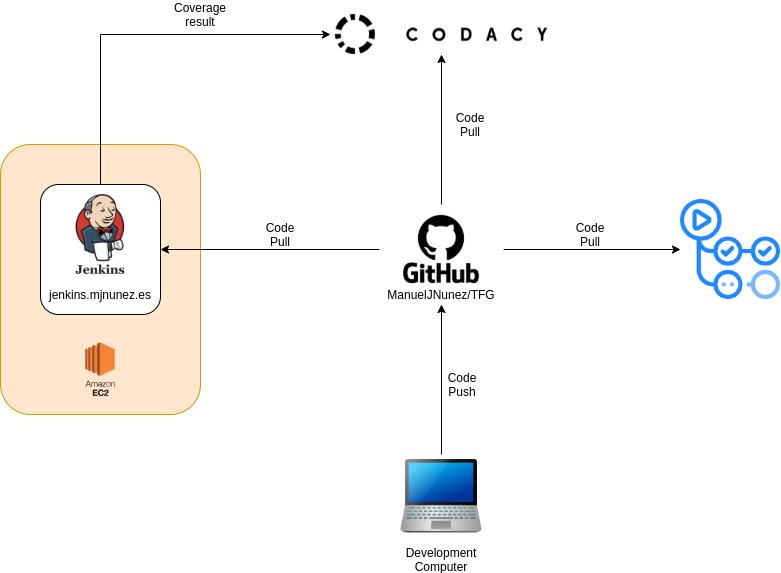
\includegraphics[width=1.\linewidth]{imagenes/05_Implementacion/testinfra.png}
	\centering
	\caption{Esquema de la infraestructura de testing usada en este trabajo.}
\end{figure}

En la imagen de arriba se puede ver la infraestructura virtual para testing que he implementado para llevar a cabo la realización de este proyecto. En esta sección, voy a proceder a describirla por partes:\newline

\begin{itemize}
	\item \textbf{Jenkins.} esta plataforma de CI ha sido alojada en AWS EC2 a través de \textit{Terraform}. El pipeline de Jenkins consta de varios \textit{stages}: el primero instala la dependencias del proyecto, luego se divide en dos caminos paralelos, uno que ejecuta los linters (\textit{Pylint} y \textit{Black}) y otro que ejecuta los tests y envía el resultado de los tests de cobertura a \textit{codacy}.

	\begin{figure}[H]
		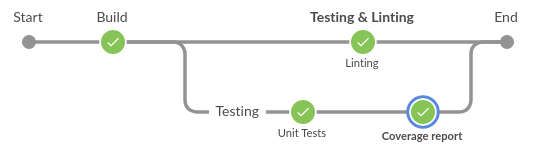
\includegraphics[width=.6\linewidth]{imagenes/05_Implementacion/jenkinspipeline.png}
		\centering
		\captionsetup{justification=centering}
		\caption{Esquema de la infraestructura de testing usada en este trabajo.}
		\label{fig:jenkinspipeline}
\end{figure}

	\item \textbf{Codacy.} esta plataforma se encarga de analizar el código y de guardar los resultados de los tests de cobertura enviados desde Jenkins. Después de analizar el código, muestra los issues del mismo, la complejidad y el porcentaje de código duplicado y le otorga una puntuación desde A hasta F, siendo A la más alta.
	
	\item \textbf{GitHub Actions.} esta plataforma ha sido usada para comprobar la ortografía del README.md, comprobar que no han sido eliminados los ficheros LICENSE, README.md y .gitignore y por último, para probar a ejecutar los tests del código en distintas versiones del intérprete de \textit{Python}, para asegurarme de la versión mínima y máxima en la que se pueden ejecutar los experimentos. 
\end{itemize}

\subsection{Integrando Jenkins con GitHub}

Cuando se usa \textit{Jenkins}, no solo basta con diseñar un \textit{pipeline}. También hay que integrarlo con GitHub para que envíe información sobre el resultado de todos los tests realizados. Esta información se envía en forma de \textit{check}.

\begin{figure}[H]
	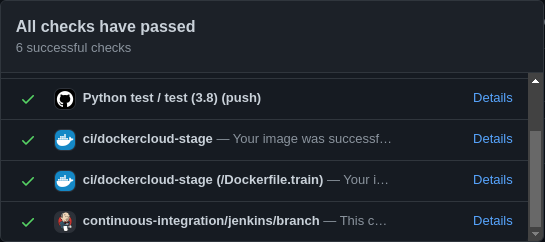
\includegraphics[width=.7\linewidth]{imagenes/05_Implementacion/ghchecks.png}
	\centering
	\caption{Checks en un commit de GitHub.}
	\label{fig:ghchecks}
\end{figure}

Por su parte, \textit{Jenkins} ofrece un plugin muy popular llamado \textit{Open Blue Ocean}, que además de incluir una interfaz web mucho más moderna e intuitiva que la de por defecto, hace uso de otros plugins para integrarse de forma fácil con \textit{GitHub}. Uno de los plugins de los que hace uso se llama \textit{GitHub}, el cual añade un webhook en \textit{Jenkins} para que cada vez que se suban cambios al repositorio, se envíe una notificación para que arranque la \textit{build} automáticamente. Otra \textit{feature} que añade es la de crear \textit{checks} para el commit en el que se está haciendo la \textit{build}.\newline

Para crear el \textit{check}, es necesario autentificar la instancia de \textit{Jenkins} en \textit{GitHub} de alguna manera. Una forma es creando un \textit{Personall Acess Token} en \textit{GitHub}, el problema de esto es que dicha instancia se autentificará como si fuera yo y por tanto usará mi imagen de perfil en los \textit{checks}. ¿Qué ocurre si en la imagen queremos indicar que el \textit{check} ha sido creado por un \textit{Jenkins}? \textit{GitHub} nos ofrece una \textit{feature} para poder integrarlo con plataformas externas, como por ejemplo las de CI/CD. Esto último se llama \textit{GitHub App}, en la cual podemos hacer que reaccione ante los eventos que queramos (\textit{push}, \textit{Pull Request}, nueva \textit{issue}) y notificas a través de una webhook a la plataforma para que reaccione a dichos eventos. Para que eso funcione, debemos de instalarla en el repositorio en el que estemos trabajando. Como se puede ver en la imagen \ref{fig:ghchecks}, uso una imagen del logo de \textit{Jenkins} para indicar el \textit{check} de dicha plataforma.\\

\subsection{Infraestructura de entrenamiento}

\begin{figure}[H]
	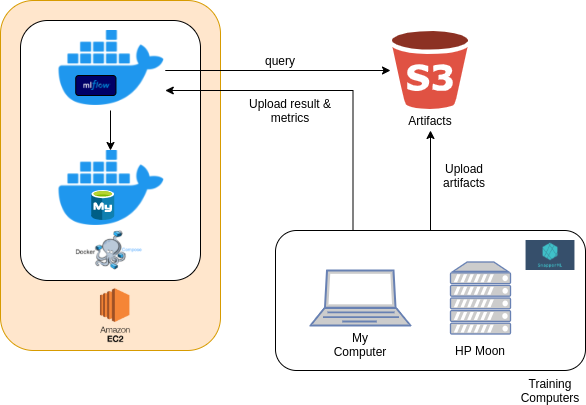
\includegraphics[width=1.\linewidth]{imagenes/05_Implementacion/traininfra.png}
	\centering
	\caption{Esquema de la infraestructura de testing usada en este trabajo.}
\end{figure}

Mi objetivo principal a la hora de realizar la infraestructura de entrenamiento es que la misma se pueda reproducir sólo con unas pocas órdenes, indicadas en el README del repositorio y también en este documento. Esta infraestructura es en realidad muy simple, consta de una instancia de EC2 y un bucket en S3 para guardar artefactos. Por otra parte, el entrenamiento se puede realizar en la máquina directamente teniendo las dependencias instaladas en un entorno virtual gestionado por \textit{poetry} o se puede entrenar usando un contenedor docker si la máquina tiene instalada la herramienta \textit{nvidia-docker2} \cite{nvidiadocker}.\newline

La máquina de EC2 que ejecuta \textit{MLFlow} está aprovisionada con \textit{terraform}, por lo que es perfectamente reproducible. Básicamente, en esta máquina se instala \textit{docker} y \textit{docker-compose} y posteriormente se copian dos ficheros (un \textit{Dockerfile}, un \textit{docker-compose.yml} y un fichero \textit{.env} que contiene la configuración necesaria) que contienen definidos la composición de servicios necesarios para ejecutar \textit{MLFlow}.\newline

En un principio había intentando usar \textit{podman} y \textit{podman-compose}, pero este último no está a la altura de su competidor aún, pues tiene varios problemas y entre ellos el que a mi me acabó afectando fue al no poder crear volúmenes, pues me daba una excepción que yo no podía controlar como usuario, debido a que el código interno de esta herramienta estaba pasando demasiados argumentos a la orden de crear volúmenes, cosa que con \textit{docker-compose} no pasaba. Tal vez \textit{podman} actualizara esa orden, pero no se actualizó en \textit{podman-compose}.\newline

Unos párrafos más atrás, he comentado que para aprovisionar la instancia de \textit{MLFlow}, hace falta un fichero \textit{.env} dentro de \textit{terraform/mlflow/}, dicho fichero debe contener las siguientes claves:

\begin{itemize}
	\item \textbf{MYSQL\_RANDOM\_ROOT\_PASSWORD.} Genera una password aleatoria para el usuario root de la base de datos, por lo que se le debe de asignar cualquier valor (pues será ignorado). También puedes asignarla tú usando la variable MYSQL\_ROOT\_PASSWORD o dejarla vacía usando MYSQL\_ALLOW\_EMPTY\_PASSWORD (inseguro).
	\item \textbf{MYSQL\_USER.} Nombre de usuario no root para acceder a la base de datos. Ejemplo: \textit{mlflow\_user}.
	\item \textbf{MYSQL\_DATABASE.} Nombre de la base de datos que contendrá toda la información sobre los experimentos registrados por mlflow. Ejemplo: \textit{mlflow\_db}.
	\item \textbf{MYSQL\_PASSWORD.} Contraseña para la base de datos que contendrá la información de mlflow. Ejemplo: \textit{mlflow\_pass}.
	\item \textbf{MYSQL\_PORT.} Puerto en el que escuchará el servicio MySQL, en el docker-compose.yml está definido en el 3306, por lo que si se pone uno distinto a ese, se debe actualizar también el otro fichero.
	\item \textbf{MLFLOW\_DBHOST.} Debe contener el valor \textit{mlflow-db}, pues así se llama el servicio de MySQL en el \textit{docker-compose.yml}.
	\item \textbf{MLFLOW\_ARTIFACTS\_URI.} URI en el que se guardarán los artefactos, puede ser local o una dirección de S3 \cite{mlflowtracking}. Ejemplos: \textit{file:///home/mjnunez/mlflow} o \textit{s3://your-bucket/path/to/artifacts}.
	\item \textbf{AWS\_ACCESS\_KEY\_ID.} Si se está usando S3, esto es necesario para la autentificación a la hora de consultar los artefactos.
	\item \textbf{AWS\_SECRET\_ACCESS\_KEY.} Si se está usando S3, esto es necesario para la autentificación, al igual que la clave anterior.
\end{itemize}

Una vez lista la configuración en el fichero, se puede desplegar en una instancia EC2 tan solo escribiendo la orden \textit{terraform apply}.\newline

Para reproducir los experimentos, caben dos posibilidades, o ejecutarlo usando un entorno virtual gestionado por \textit{poetry}, o ejecutarlos dentro de un contenedor que he diseñado para ese propósito (no recomendado, pues el contenedor ocupa 7.01GB). De todos modos, hay que crear otro fichero \textit{.env} en el directorio principal del proyecto con las siguientes claves:

\begin{itemize}
	\item \textbf{POSTGRES\_PASSWORD.} Contraseña para acceder a la base de datos postgres. Ejemplo: \textit{tu-clave123}.
	 \item \textbf{POSTGRES\_USER.} Nombre de usuario para acceder a la base de datos. Ejemplo: \textit{user123}.
	 \item \textbf{POSTGRES\_DB.} Nombre de la base de datos dónde optuna guardará sus datos. Ejemplos: \textit{optuna}.
	 \item \textbf{MLFLOW\_TRACKING\_URI.} dirección URL (o IP) de tu servicio mlflow. Ejemplos: \textit{http://localhost} o \textit{http://mlflow.tu-dominio.com}.
	 \item \textbf{OPTUNA\_STORAGE\_URI.} URI para acceder a la base de datos \textit{posgres}.
	 \item \textbf{AWS\_ACCESS\_KEY\_ID.} Si se está usando S3 en la instancia de \textit{MLflow} para guardar los artefactos, esto es necesario para la autentificación a la hora de subir los artefactos. También se pueden configurar en \textit{$\sim$/.aws/credentials}.
	 \item \textbf{AWS\_SECRET\_ACCESS\_KEY.} Al igual que la variable anterior, sirve para esto es necesario para la autentificación a la hora de subir artefactos. También se pueden configurar en \textit{$\sim$/.aws/credentials}.
\end{itemize}

Una vez configurado todo, podemos arrancar los experimentos con la orden \textit{poetry run inv venvtrain} para ejecutarlo usando los paquetes del entorno virtual de \textit{Python} o usando \textit{poetry run inv dockertrain} para ejecutar los experimentos dentro de un contenedor. A parte de lo anterior, se puede entrenar en otra máquina usando el entorno virtual (en mi caso el HPMoon) a través de SSH usando la siguiente orden:

\begin{lstlisting}[language=bash]
$ poetry run inv sshtrain --destdir=<destination_directory> --host=<server_dir> [--gw=<gw_dir>].
\end{lstlisting}

Sobre la imagen base del contenedor, mi objetivo era que tuviera soporte para usar también GPUs dentro del mismo. Por este mismo motivo, al principio usé \textit{nvidia/cuda:11.3.0-cudnn8-devel-ubuntu20.04}, con la cual terminaba obteniendo una imagen de más de 10GB que no podía construir ni descargar desde un repositorio de contenedores en el HP Moon. Esto era debido a que el tamaño máximo que podía ocupar un contenedor en dicha máquina estaba limitado a 10GB, pero por una petición que le hice al administrador se amplió hasta 20GB. Esto último al final no sirvió, debido a que al final acabé usando una imagen más ligera llamada \textit{nvidia/cuda:11.3.0-cudnn8-runtime-ubuntu20.04}, que también trae las \textit{CUDA math libraries} e incluye \textit{cuDNN}, una biblioteca acelerada por GPU que provee de implementaciones para rutinas estándar como por ejemplo para la \textit{backward propagation} y la \textit{forward propagation}. Esta última es la que usa \textit{PyTorch} a la hora de entrenar modelos por GPU \cite{cudnn}. Como indiqué anteriormente, el tamaño final del contenedor es de 7,01GB.\\

\subsection{Buenas prácticas seguidas a la hora de diseñar los contenedores}\label{subsec:dockerpractices}

A la hora de realizar el proyecto, me he preocupado de seguir las mejores prácticas posibles a la hora de diseñar los \textit{Dockerfiles}. Una de las cosas que más me ha importado ha sido elegir la imagen base más pequeña \cite{dockerbestpracticesdev} (en la subsección anterior ya hablo un poco sobre esto con la imagen de \textit{nvidia/cuda}), por eso en la mayoría de contenedores he usado \textit{python:3.8-slim}. Hay otra imagen más ligera aún que esa llamada \textit{python:3.8-alpine} pero no trae muchas herramientas instaladas y siempre el \textit{workaround} usando estas imágenes es mayor que con otras y suelen acabar ocupando solo un poco menos, por lo que en esta ocasión no compensa tanto ese \textit{workaround}. El uso de esta práctica es necesario para terminar con imágenes finales de poco tamaño y que se puedan ser descargadas en poco tiempo.\newline

Otra práctica interesante que he puesto en práctica también para reducir el volumen de la imagen final, es eliminar la caché del gestor de los gestores de paquetes. Y una que no podemos dejar atrás, reducir el número de capas. Con esto quiero decir que debemos usar el menor número de instrucciones \textit{RUN}, \textit{COPY} y \textit{ADD} que son las que crean las capas. Usarlas frecuentemente implica que el tamaño de la imagen final sea mayor. Por eso, es recomendable encadenar varias órdenes dentro de un mismo \textit{RUN} y así solo se crearía una capa \cite{dockerbestpractices}.\newline

En cuanto a la seguridad del contenedor, siempre es conveniente no usar el usuario \textit{root} que viene por defecto en todos las imágenes de contenedores. Esto es debido a que en caso de un ataque, la superficie sería mayor que usando un usuario que tenga solo acceso a lo justo y necesario, es decir, la aplicación que funcione dentro del contenedor \cite{dockerbestpracticesdev}.\newline

Una buena práctica general de los contenedores es usar cada contenedor para un único propósito. Si desacoplamos aplicaciones entre varios contenedores, el escalado horizontal y el reusar la imagen se hacen más fáciles \cite{dockerbestpractices}.

%
\chapter{Experimentación}

En este capítulo se van a exponer todas las pruebas realizadas sobre los \textit{scripts} de entrenamiento. Estas pruebas van desde \textit{profiling} de memoria hasta la prueba de entrenamiento de los modelos usando distintos hiperparámetros. De estos últimos se realizará un análisis para conocer bien cuáles son los hiperparámetros que más influencia tienen sobre la métrica que mide la capacidad de clasificación del modelo generado.\\

Además de lo anterior, se realizará una comparación entre los mejores resultados obtenidos en cada experimento y una comparación del uso de memoria.\\

Me gustaría también agradecer a las personas del \textit{Southern Wide-field Gamma-ray Observatory} (\textit{SWGO}) y del \textit{Laboratório de Instrumentação e Física Experimental de Partículas} (\textit{LIP}), más concretamente a Mario Pimenta, Ruben Conceição y Bernardo Tomé, por proveerme del conjunto de datos obtenido de sus simulaciones. Un análisis de estos datos se encuentra en la Seccción \ref{chap:datanalysis}.

\section{Memory profiling}

En esta sección, mostraré los resultados del \textit{profiling} de memoria realizado a todos los scripts de entrenamiento para saber cuánta memoria usan y por tanto es necesaria para poder ejecutarlos.\\

El \textit{profiling} nos permite conocer los recursos que un \textit{software} (en este caso los \textit{script}) necesita. Hoy en día tenemos la suerte de que los componentes de un computador decente está al alcance de casi todos (excepto las \textit{GPU}s cuando hay un \textit{boom} de criptomonedas). Pero si los componentes son accesibles económicamente para casi todo el mundo, ¿para qué hacemos \textit{profiling} entonces? Vamos a imaginar que queremos montar un computador de alto rendimiento para entrenar modelos lo más rápido posible. Tal vez la inversión más importante sea una buena \textit{GPU} por el tema de aprovechar el paralelismo que ofrece. Y ahora viene otra pregunta ¿cuánta \textit{RAM} necesitamos? Si ponemos demasiada sería un poco derroche económico pero si nos quedamos cortos se usaría memoria alocada en el disco duro (\textit{SWAP}) que es mucho más lenta que la \textit{RAM} y por tanto ralentizaría nuestras ejecuciones. Si sabemos la cantidad de \textit{RAM} que consumen nuestros \textit{scripts} o \textit{software} podemos conocer la cantidad de memoria que vamos a necesitar en nuestro computador.\\

También sería conveniente analizar cuanta memoria usa nuestro modelo una vez desplegado de nuevo para hacer la inversión correcta en memoria \textit{RAM}. Pero la cosa no queda ahí, ¿Y si queremos desplegar nuestro modelo en un dispositivo empotrado\footnote{Los dispositivos empotrados (como por ejemplo \textit{Arduino}, \textit{ESP32} o \textit{ARM}) normalmente tienen recursos muy limitados (suelen tener por lo general unos pocos KiBs o MiBs de RAM) y poco uso de energía, pues suelen funcionar con baterías y nos interesa que estas duren lo máximo posible.}? En este caso nos estamos refiriendo al campo del \textit{tinyML}. Estos dispositivos no suelen tener una gran cantidad de memoria (no suelen llegar ni al medio GiB) por tanto en estos casos también nos interesa usar \textit{profiling} e intentar optimizar lo máximo posible el uso de memoria y \textit{CPU}\footnote{En el caso del \textit{tinyML} también sería interesante el uso de un \textit{profiler} de \textit{CPU}.} para ahorrar la máxima batería posible. Para este caso de uso existen librerías de \textit{Machine Learning} más ligeras como \textit{PyTorch Lite} o \textit{TensorFlow Lite}.\\

Ya hemos hablado del \textit{tinyML}, pero ¿sería interesante también tener en cuenta el uso de memoria en el contexto de \textit{Edge Computing}? En este caso, tendríamos sensores que publican datos en \textit{streaming} o publican estados de algún objeto en tiempo real y un computador que se subscribe a los datos para analizarlos en tiempo real o enviarlos a la \textit{cloud} de una gran empresa para usarlos en futuras mejoras del sistema. Estos sensores y dicho computador tal vez están manejando un vehículo autónomo con una familia dentro. Si dicho computador que controla el vehículo se queda corto de memoria podría dejar de responder a los estímulos externos en tiempo real y producirse una catástrofe. Con esto quiero recalcar que es esencial el uso de \textit{profiling} en sistemas críticos.\\

En conclusión, en estos párrafos anteriores se deja demostrada la importancia del \textit{profiling} a la hora de diseñar sistemas que vayamos a desplegar en algún dispositivo ya sea empotrado o no y la esencialidad del mismo a la hora del diseño de sistemas críticos que puedan llevar a la pérdida de vidas humanas.\\

\subsection{Memory profiling para \textit{Convolutional Autoencoder}}

El modelo que ha sido perfilado en esta sección ha sido descrito en la Sección \ref{subsec:cae}.

\begin{figure}[H]
	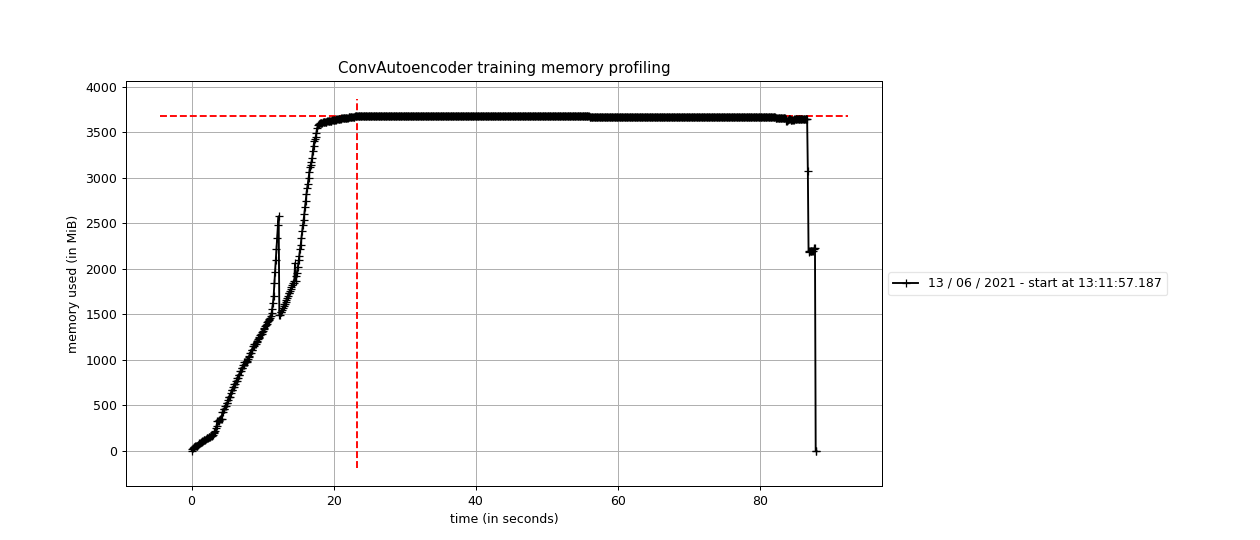
\includegraphics[width=1.\linewidth]{imagenes/06_Experimentacion/cae.png}
	\centering
	\caption{Gráfico de uso de memoria del script de entrenamiento de entrenamiento para el ConvAutoencoder (\path{src/cae.py}).}
\end{figure}

Al principio, puede observarse una subida muy pronunciada debido a la lectura del dataset (ocupa aproximadamente 1500 MiB en memoria). A parte, también se puede observar otra gran subida producida al cargar el modelo de \textit{Machine Learning} en la GPU. El uso total de memoria de este script es de 3650.3 MiB, aproximadamente 3.56 GiB.\\

\subsection{Memory profiling para \textit{Convolutional Classifier}}

El modelo que ha sido perfilado en esta sección ha sido descrito en la Sección \ref{subsec:convnet}.

\begin{figure}[H]
	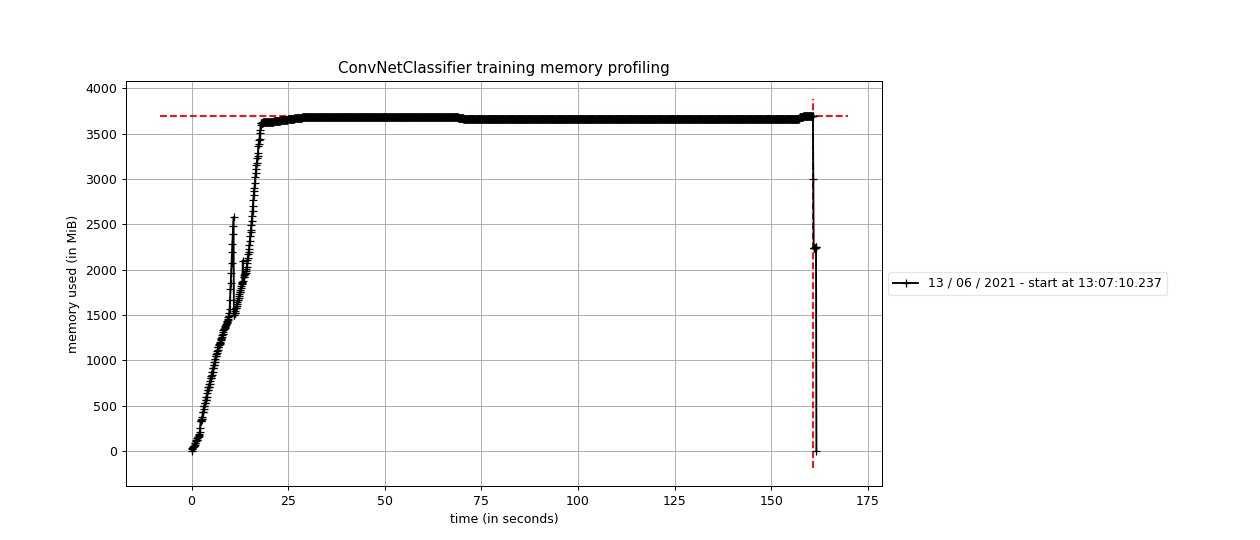
\includegraphics[width=1.\linewidth]{imagenes/06_Experimentacion/convnet.png}
	\centering
	\caption{Gráfico de uso de memoria del script de entrenamiento de entrenamiento para el ConvClassifier (\path{src/convnet.py}).}
\end{figure}

El máximo de memoria requerida durante la ejecución del script de entrenamiento es de 3693.7 MiB, aproximadamente 3.61GiB. En este caso, las subidas son debidas a la lectura del dataset y a la carga del modelo en la GPU.\\

\subsection{Memory profiling para \textit{ResNet}}

El modelo que ha sido perfilado en esta sección está descrito en la anterior Sección \ref{subsec:resnet}.

\begin{figure}[H]
	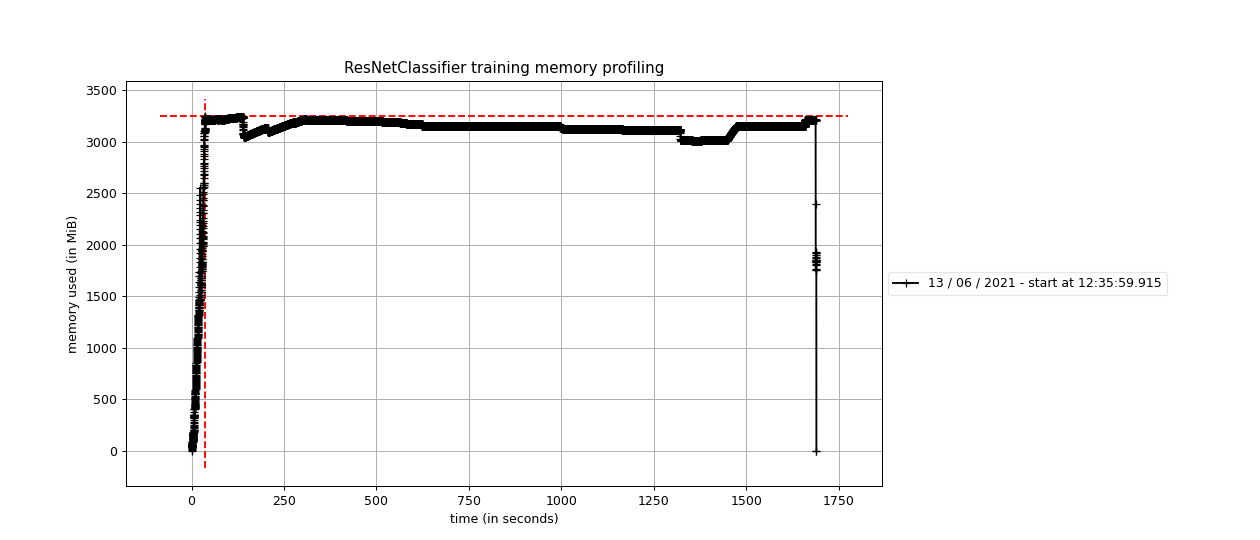
\includegraphics[width=1.\linewidth]{imagenes/06_Experimentacion/resnet.png}
	\centering
	\caption{Gráfico de uso de memoria del script de entrenamiento de entrenamiento para el ResNetModel (\path{src/resnet.py}).}
\end{figure}

Este script requiere menos memoria para poder ejecutarse en condiciones que los demás, pues requiere 3214.6 MiB, aproximadamente 3.14 GiB. El incremento de uso en memoria es debido a, como en las Subsecciones anteriores, la carga del dataset y la carga del modelo en GPU.\\

\subsection{Memory profiling para \textit{Varitional Autoencoder}}

El modelo que ha sido perfilado en esta sección está descrito en la anterior Sección \ref{subsec:vae}.

\begin{figure}[H]
	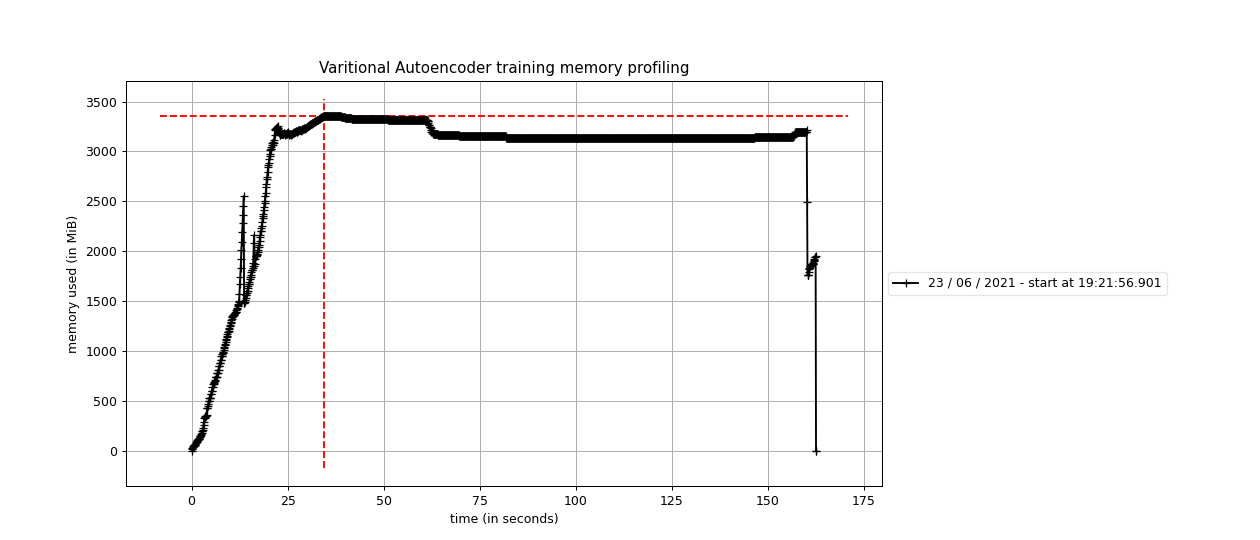
\includegraphics[width=1.\linewidth]{imagenes/06_Experimentacion/vae.png}
	\centering
	\caption{Gráfico de uso de memoria del script de entrenamiento de entrenamiento para el Varitional Autoencoder (\path{src/vae.py}).}
\end{figure}

El script de entrenamiento del Varitional Autoencoder requiere 3223.1 MiB de memoria, aproximadamente 3.15 GiB. Las partes del script que más han incrementado el uso de memoria coincide con los otros experimentos que han sido perfilados en las Subsecciones anteriores.\\

\subsection{Comparativa final del uso de memoria}

\begin{table}[H]
\centering
\begin{tabular}{cc}
\hline
\textbf{Script}                    & \textbf{Uso de memoria} \\ \hline
\path{src/cae.py}                  & 3.56 GiB                \\ \hline
\path{src/convnet.py}              & 3.61 GiB                \\ \hline
\path{src/resnet.py}               & 3.14 GiB                \\ \hline
\path{src/vae.py}                  & 3.15 GiB                \\ \hline
\end{tabular}
\caption{Resultados globales del \textit{profiling} de memoria.}
\label{tab:memoryprofile}
\end{table}

Como se puede ver en la Tabla \ref{tab:memoryprofile}, el script que más memoria consume es el que se encuentra en \path{src/convnet.py}, pero el que se encuentra en \path{src/cae.py} consume casi lo mismo. Los otros dos scripts consumen en torno a los 3.15 GiB. El tamaño de memoria que le pondría a una máquina de entrenamiento para este conjunto de datos sería de un mínimo de 8GiB\footnote{Usando dos módulos de 4 GiB idénticos para aprovechar las ventajas del \textit{Dual Channel}.}, pues hay que dejar espacio para las rutinas del SO y con 4GiB se quedaría corto.

\section{Configuración de las pruebas de diseño}

En esta Sección se va a presentar la configuración de todos los experimentos implementados y el rango de valores que puede tomar sus hiperparámetros junto con la distribución de los mismos.\\

\subsection{Configuración común entre experimentos}

\textit{SnapperML} no permite establecer un fichero de configuración con variables globales, lo que me refiero en esta Subsección con configuración global es a variables que he usado en todos los experimentos con los mismos valores.\\

\setlength{\tabcolsep}{10pt} % Default value: 6pt
\renewcommand{\arraystretch}{1.5} % Default value: 1

\begin{table}[h]
\centering
\begin{tabular}[c]{m{3cm}m{3cm}}
\hline
\textbf{Variable} & \textbf{Valor} \\ \hline
epochs            & 5              \\
seed              & 2342           \\ \hline
\end{tabular}
\caption{Configuración global para todos los experimentos.}
\label{tab:globalvalues}
\end{table}

En la Tabla \ref{tab:globalvalues} quiero decir que todos los modelos creados en los experimentos se entrenan durante 5 épocas (entendidas estas como un pase completo por todos los \textit{batches} del conjunto de datos) y se inicializa el generador aleatorio de \textit{PyTorch} con la semilla 2342. Aunque 5 épocas parezca poco, ya se pueden obtener buenos resultados (véase Tabla \ref{tab:results}).

\subsection{Configuración \textit{Convolutional Autoencoder}}

Los hiperparámetros de este modelo han sido exlicados en la Subsección \ref{subsec:cae}. En este experimento, se usa el modelo introducido en la Subsección \ref{subsub:convautoencoder}. Con este modelo se puede realizar una reducción de dimensionalidad de los datos para aprender de datos simplificados en lugar de los originales. Por esa razón es un modelo interesante para experimentar.\\

\begin{table}[H]
\centering
\begin{tabular}[c]{m{6cm}m{3cm}}
\hline
\textbf{Variable}                 & \textbf{Valor}  \\ \hline
Nombre del experimento            & CAE             \\
Número de configuraciones         & 1               \\ \hline
\end{tabular}
\caption{Información general sobre el experimento \textit{Convolutional Autoencoder}.}
\label{tab:caeinfo}
\end{table}

\begin{table}[H]
\centering
\begin{tabular}{m{4cm}m{5.1cm}}
\hline
\textbf{Variable}                 & \textbf{Valor}                          \\ \hline
\textit{Batch Size}               & randint(32,256)                         \\
\textit{Learning rate}            & loguniform(0.0001, 0.01)                \\
\textit{Regularization}           & loguniform(0.0001, 0.1)                 \\
Canales de salida en la primera convolución &   randint(1, 10)              \\
Profundidad                       & randint(1,4)                            \\
Tamaño del código latente         & randint(10, 100)                        \\
Optimizador                       & choice(['adam', 'sgd'])                 \\ \hline
\end{tabular}
\caption{Hiperparámetros para el experimento \textit{Convolutional Autoencoder}.}
\label{tab:caeconfig}
\end{table}

En este y en todos los siguientes experimentos se ha probado con un \textit{batch size} variable para ver si afecta al resultado final o no. Además, también se ha probado con un \textit{learning rate} y con un valor de regularización que toman valores en un rango amplio. También pruebo con dos optimizadores para compararlos, \textit{Adam} (explicado en la Subsección \ref{subsec:learningalgorithms}) y \textit{SGD} (explicado en la misma Subsección).\\

Además, he experimentado con varios valores para el número de canales de salida en la primera convolución (tomando valores entre 1 y 10), con varios valores para la profundidad del \textit{encoder} y del \textit{decoder} (de 2 a 4, pues si toma un valor mayor el tamaño de la imagen sería aproximadamente de 2x2 y se usan \textit{kernels} de 3x3 en las operaciones convolucionales). Por último, he probado también con varios valores para el tamaño del código latente (de 10 a 100).\\

\subsection{Configuración \textit{Convolutional Classifier}}

Los hiperparámetros de este modelo han sido exlicados en la Subsección \ref{subsec:convnet}. En resumen a dicha Subsección, en este experimento se prueba con una red convolucional basasda en \textit{LeNet-5} (un modelo bastante simple pero con buenos resultados) con un número de canales de salida variable para cada convolución para que con \textit{optuna} se encuentre la mejor combinación posible que maximice la métrica objetivo.\\

\begin{table}[H]
\centering
\begin{tabular}[c]{m{6cm}m{3cm}}
\hline
\textbf{Variable}                 & \textbf{Valor}  \\ \hline
Nombre del experimento            & Simple CNN      \\
Número de configuraciones         & 1               \\ \hline
\end{tabular}
\caption{Información general sobre el experimento \textit{Convolutional Classifier}.}
\label{tab:convnetinfo}
\end{table}

\begin{table}[H]
\centering
\begin{tabular}{m{3cm}m{5.1cm}}
\hline
\textbf{Variable}                 & \textbf{Valor}                          \\ \hline
\textit{Batch Size}               & randint(32,256)                         \\
\textit{Learning rate}            & loguniform(0.0001, 0.01)                \\
Optimizador                       & choice(['adam', 'sgd'])                 \\ 
Output channels                   & randint(2, 20) $\times$ randint(2, 20)  \\ \hline
\end{tabular}
\caption{Hiperparámetros para el experimento \textit{Convolutional Classifier}.}
\label{tab:convnetconfig}
\end{table}

La última diferencia que tiene este experimento con el anterior es que se genera una \textit{List} aleatoria para probar con distintos valores de canales de salida de las capas convolucionales y ver como afecta a las métricas.\\

\subsection{Configuración \textit{ResNet}}\label{subsec:resnet}

Los hiperparámetros de este modelo han sido exlicados en la Subsección \ref{subsec:resnetarch}. En resumen a dicha Subsección, se va a usar una implementación basada en \textit{ResNet}, una red convolucional muy popular en el campo de clasificación de imágenes y por tanto con una gran capacidad de clasificación (tal vez de las mejores). Este caso particular de \textit{ResNet} tiene un número de canales para cada grupo de \textit{ResBlocks} variable y el número de \textit{ResBlocks} en cada grupo también es variable.\\

\begin{table}[H]
\centering
\begin{tabular}[c]{m{6cm}m{3cm}}
\hline
\textbf{Variable}                 & \textbf{Valor}  \\ \hline
Nombre del experimento            & ResNet          \\
Número de configuraciones         & 1               \\ \hline
\end{tabular}
\caption{Información general sobre el experimento \textit{ResNet}.}
\label{tab:resnetinfo}
\end{table}

\begin{table}[H]
\centering
\begin{tabular}{m{3cm}m{7cm}}
\hline
\textbf{Variable}                 & \textbf{Valor}                          \\ \hline
\textit{Batch Size}               & randint(32,256)                         \\
\textit{Learning rate}            & loguniform(0.0001, 0.01)                \\
\textit{Regularization}           & loguniform(0.0001, 0.1)                 \\
Optimizador                       & choice(['adam', 'sgd'])                 \\ 
Número de bloques                 & randint(2, 6) $\times$ randint(2, 6) $\times$ randint(2, 6) $\times$ randint(2, 6) \\
Número de canales                 & randint(8, 32) $\times$ randint(32, 64) $\times$ randint(64, 128) $\times$ randint(128, 256) $\times$ randint(256, 512) \\
\hline
\end{tabular}
\caption{Hiperparámetros para el experimento \textit{ResNet}.}
\label{tab:resnetconfig}
\end{table}

El número de bloques toma un valor entre 2 y 6 porque tampoco quiero que el modelo sea muy profundo (y por tanto tarde demasiado tiempo en ajustarse a los datos de entrenamiento). El número de canales va aumentando conforme vamos profundizando en la red, tal y como sucede en el modelo original.

\subsection{Configuración \textit{Varitional Autoencoder}}

Los hiperparámetros de este modelo han sido exlicados en la Subsección \ref{subsec:vae}. Este modelo no usa ninguna capa convolucional y por eso mismo es interesante experimentar con él, para compararlo con otros modelos convolucionales. Como se ha especificado en la Subsección de antes, este modelo tiene el número de neuronas por capa variable, permitiendo a \textit{optuna} encontrar aquel que maximice la métrica objetivo.\\

\begin{table}[H]
\centering
\begin{tabular}[c]{m{6cm}m{3cm}}
\hline
\textbf{Variable}                 & \textbf{Valor}  \\ \hline
Nombre del experimento            & ResNet          \\
Número de configuraciones         & 1               \\ \hline
\end{tabular}
\caption{Información general sobre el experimento \textit{Varitional Autoencoder}.}
\label{tab:resnetinfo}
\end{table}

\begin{table}[H]
\centering
\begin{tabular}{m{3cm}m{7cm}}
\hline
\textbf{Variable}                 & \textbf{Valor}                          \\ \hline
\textit{Batch Size}               & randint(32,256)                         \\
\textit{Learning rate}            & loguniform(0.0001, 0.01)                \\
\textit{Regularization}           & loguniform(0.0001, 0.1)                 \\
Optimizador                       & choice(['adam', 'sgd'])                 \\ 
Tamaño de las capas               & randint(500, 1000) $\times$ randint(100, 500) $\times$ randint(50, 100) $\times$ randint(10, 50) \\
\hline
\end{tabular}
\caption{Hiperparámetros para el experimento \textit{Varitional Autoencoder}.}
\label{tab:resnetconfig}
\end{table}

\section{Resultados}

En esta sección se presentan los resultados obtenidos de la ejecución de los experimentos anteriores. La métrica usada para seleccionar al mejor ha sido la \textit{$F_1$ score}. Para calcular esta métrica, se hace uso de otras dos, la \textit{precision} y el \textit{recall}.\\

En una clasificación binaria, podemos clasificar las predicciones tal que así:

\begin{table}[H]
\centering
\begin{tabular}{c|c|c|}
\cline{2-3}
 &
  \textbf{\begin{tabular}[c]{@{}c@{}}Predicción\\ Positivo\\ (y=1)\end{tabular}} &
  \textbf{\begin{tabular}[c]{@{}c@{}}Predicción\\ Negativo\\ (y=0)\end{tabular}} \\ \hline
\multicolumn{1}{|c|}{\textbf{\begin{tabular}[c]{@{}c@{}}Positivo\\ (y=1)\end{tabular}}} &
  \begin{tabular}[c]{@{}c@{}}Verdaderos\\ Positivos\end{tabular} &
  \begin{tabular}[c]{@{}c@{}}Falsos\\ Negativos\end{tabular} \\ \hline
\multicolumn{1}{|c|}{\textbf{\begin{tabular}[c]{@{}c@{}}Negativo\\ (y=0)\end{tabular}}} &
  \begin{tabular}[c]{@{}c@{}}Falsos\\ Positivos\end{tabular} &
  \begin{tabular}[c]{@{}c@{}}Verdaderos\\ Negativos\end{tabular} \\ \hline
\end{tabular}
\caption{Clasificación de las predicciones.}
\label{tab:predictions}
\end{table}

\begin{align}
	&Precision = \frac{True Positives}{True Positives + False Positives}\\
	&Recall = \frac{True Positives}{True Positives + False Negatives}
\end{align}

Por tanto, la \textit{precision} mide el balance entre los verdaderos positivos y lo que se predice como positivo (ya sea verdadero o falso). Por otra parte, el \textit{recall} mide el balance entre los verdaderos positivos y los positivos que han sido predecidos bien o mal. Una vez que ya sabemos como se calcula la \textit{precision} y el \textit{recall}, podemos calcular la \textit{$F_1$ score} de la forma siguiente:

\begin{align}
&F_1 score = 2 \frac{precision \cdot recall}{precision + recall}
\end{align}

En la Tabla \ref{tab:results} se muestran los resultados de los experimentos (los mejores modelos obtenidos de cada uno) y en la Figura \ref{fig:confusion} se muestran las \textit{confusion matrices} de los resultados. Como se puede observar, los resultados no son muy distintos de un experimento a otro, pues todos tienen casi el mismo \textit{$F_1$ score}. El modelo que tiene menor valor en esta métrica es el \textit{Varitional Autoencoder}, los modelos con capas convolucionales tienen mejores resultados que este último. El experimento que mejor resultado ha tenido, aunque tampoco hay mucha diferencia, ha sido el de \textit{Simple CNN} (modelo basado en LeNet-5). En las \textit{Confusion matrices} se puede observar que no hay mucha diferencia entre una y otra, pues en todos los casos son capaces de predecir bien cerca del 99\% de las muestras.\\

\begin{figure}[H]
\begin{subfigure}{.5\textwidth}
  \centering
  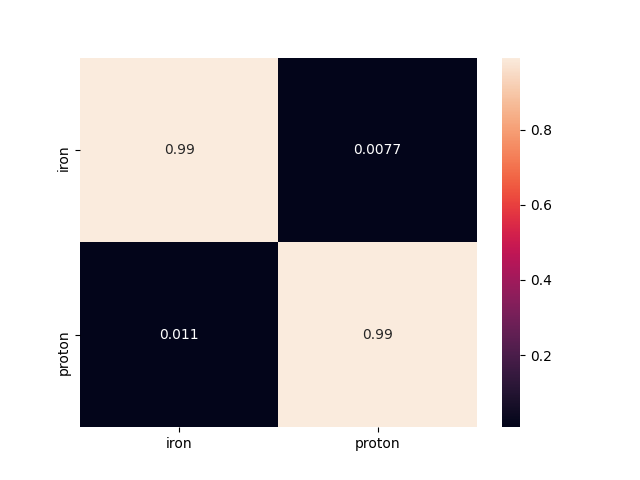
\includegraphics[width=.8\linewidth]{imagenes/06_Experimentacion/simplecnncm.png}  
  \caption{Simple CNN confusion matrix.}
  \label{fig:simplecnncm}
\end{subfigure}
\begin{subfigure}{.5\textwidth}
  \centering
  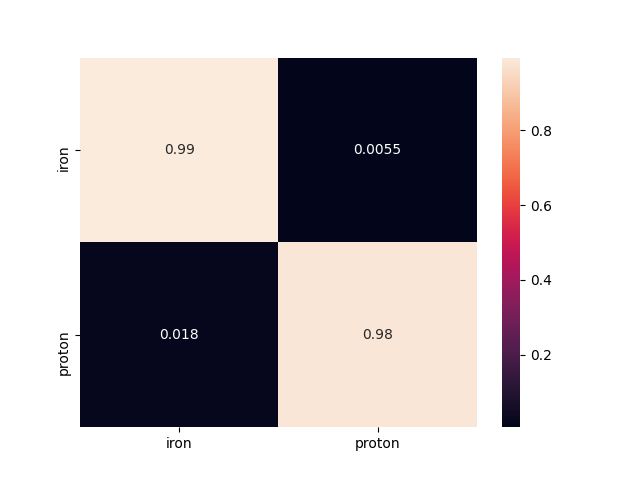
\includegraphics[width=.8\linewidth]{imagenes/06_Experimentacion/caecm.png}  
  \caption{CAE confusion matrix.}
  \label{fig:caecm}
\end{subfigure}

\newline

\begin{subfigure}{.5\textwidth}
  \centering
  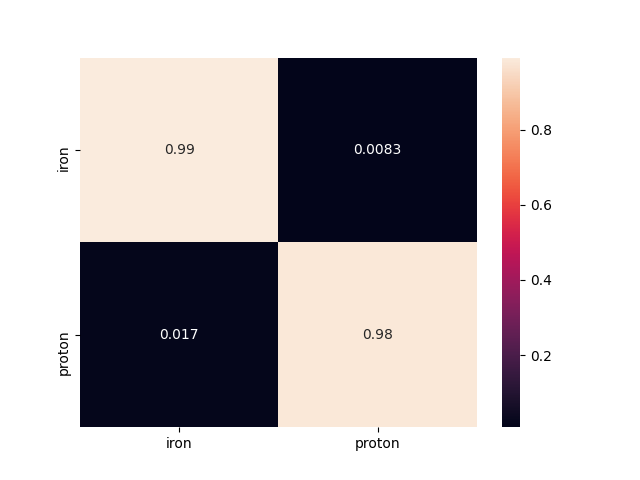
\includegraphics[width=.8\linewidth]{imagenes/06_Experimentacion/resnetcm.png}  
  \caption{ResNet confusion matrix.}
  \label{fig:resnetcm}
\end{subfigure}
\begin{subfigure}{.5\textwidth}
  \centering
  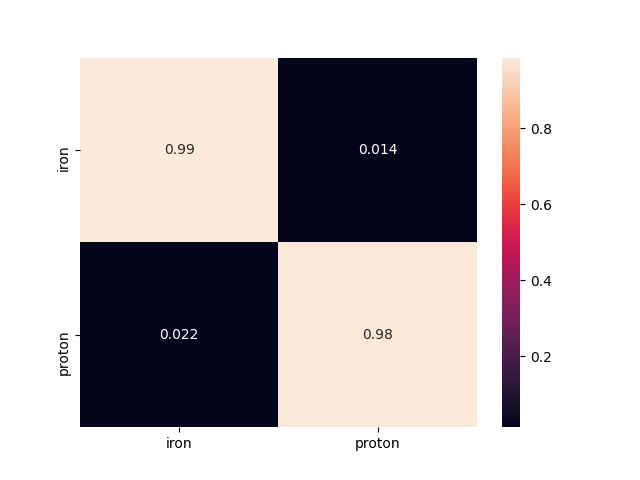
\includegraphics[width=.8\linewidth]{imagenes/06_Experimentacion/vaecm.png}  
  \caption{VAE confusion matrix.}
  \label{fig:vaecm}
\end{subfigure}
\caption{\textit{Confusion matrices} de los mejores resultados de los experimentos.}
\label{fig:confusion}
\end{figure}

\begin{table}[H]
\centering
\begin{tabular}{ccc}
\hline
\textbf{Experimento} &
  \textbf{Hiperparámetros} &
  \textbf{$\mathbf{F_1}$ score (Test)} \\ \hline
CAE &
  \begin{tabular}[c]{@{}c@{}}depth: 3\\ latent\_size: 65\\ batch\_size: 255\\ optimizer: adam\\ first\_conv\_out\_channels: 9\\ lr: 0.0029064860639852596\\ reg: 0.008171626239529795\end{tabular} &
  0.988 \\ \hline
Simple CNN &
  \begin{tabular}[c]{@{}c@{}}batch\_size: 180\\ optimizer: adam\\ out\_channels: {[}14, 18{]}\\ lr: 0.0017701827211672693\end{tabular} &
  0.991 \\ \hline
ResNet &
  \begin{tabular}[c]{@{}c@{}}batch\_size: 89\\ optimizer: sgd\\ lr: 0.0037730724227855905\\ reg: 0.0002618785645692275\\ number\_of\_blocks: {[}4, 6, 6, 5{]}\\ num\_channels: {[}14, 45, 86, 181, 430{]}\end{tabular} &
  0.987 \\ \hline
VAE &
  \begin{tabular}[c]{@{}c@{}}batch\_size: 37\\ optimizer: adam\\ lr: 0.0004440804594397368\\ reg: 0.0004545588488375805\end{tabular} &
  0.982 \\ \hline
\end{tabular}
\caption{Resultados de cada experimento}
\label{tab:results}
\end{table}

\newpage
\subsection{Análisis resultados \textit{Convolutional Autoencoder}}

\begin{figure}[H]
\begin{subfigure}{.5\textwidth}
  \centering
  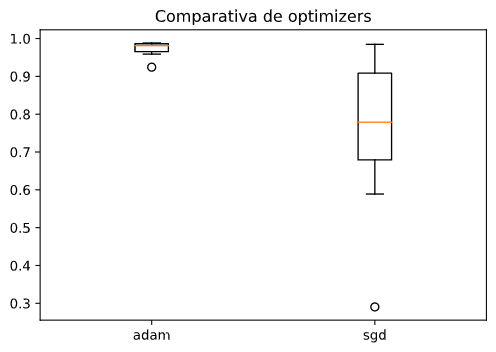
\includegraphics[width=.8\linewidth]{imagenes/06_Experimentacion/caeimages/caeoptimizers.png}
  \caption{\textit{Optimizers boxplot}.}
  \label{fig:caeoptimizers}
\end{subfigure}
\begin{subfigure}{.5\textwidth}
  \centering
  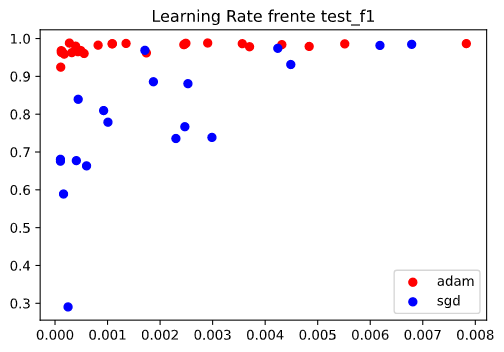
\includegraphics[width=.8\linewidth]{imagenes/06_Experimentacion/caeimages/caelr.png}  
  \caption{\textit{Learning rate} frente \textit{$F_1$ score}.}
  \label{fig:caelr}
\end{subfigure}

\newline

\begin{subfigure}{.5\textwidth}
  \centering
  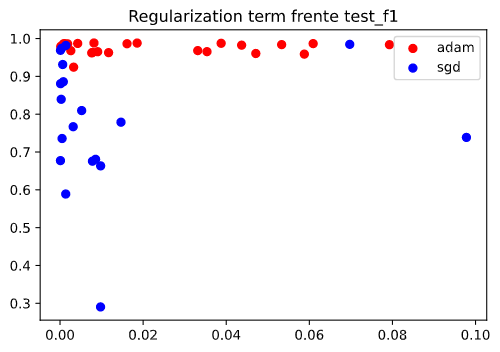
\includegraphics[width=.8\linewidth]{imagenes/06_Experimentacion/caeimages/caereg.png}
  \caption{\textit{Regularization} frente \textit{$F_1$ score}.}
  \label{fig:caeoreg}
\end{subfigure}
\begin{subfigure}{.5\textwidth}
  \centering
  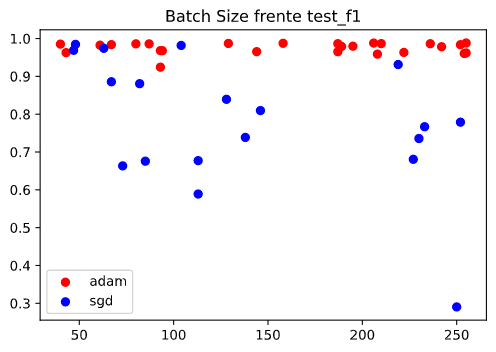
\includegraphics[width=.8\linewidth]{imagenes/06_Experimentacion/caeimages/caebs.png}  
  \caption{\textit{Batch size} frente \textit{$F_1$ score}.}
  \label{fig:caebr}
\end{subfigure}

\newline

\begin{subfigure}{.5\textwidth}
  \centering
  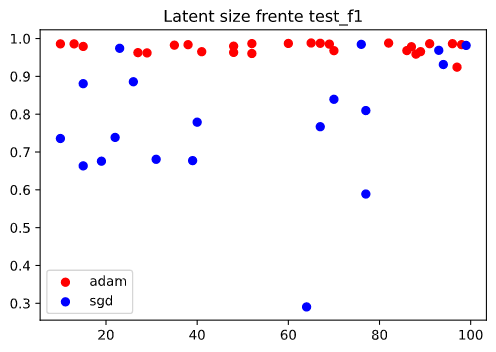
\includegraphics[width=.8\linewidth]{imagenes/06_Experimentacion/caeimages/caelatentsize.png}
  \caption{\textit{Latent Size} frente \textit{$F_1$ score}.}
  \label{fig:caelatentsize}
\end{subfigure}
\begin{subfigure}{.5\textwidth}
  \centering
  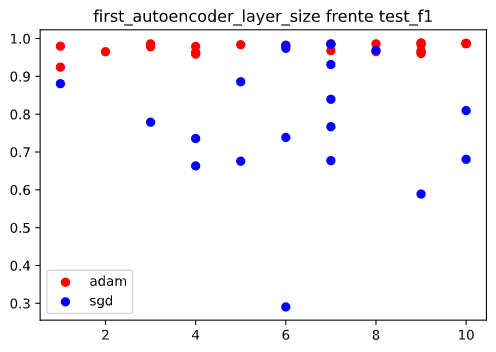
\includegraphics[width=.8\linewidth]{imagenes/06_Experimentacion/caeimages/caefcoc.png}  
  \caption{\textit{first\_autoencoder\_layer\_size} frente \textit{$F_1$ score}.}
  \label{fig:caefcoc}
\end{subfigure}

\caption{Plots para analizar del efecto de los hiperparámetros en los resultados del experimento CAE.}
\label{fig:caeanalysis}
\end{figure}

Viendo la Figura \ref{fig:caeanalysis} podemos sacar las siguientes conclusiones:

\begin{itemize}
    \item De la Figura \ref{fig:caeoptimizers} podemos sacar como conclusión que el optimizador \textit{Adam} da mejores resultados que \textit{SGD} por mucho. A parte de tener resultados mejores, estos son menos dispersos y están a la altura del Q4 de los resultados de \textit{SGD}.
    \item En la Figura \ref{fig:caelr} podemos observar que \textit{Adam} saca buenos resultados independientemente del valor del \textit{learning rate}. Sobre \textit{SGD}, parece que a más alto es el valor, mejores resultados saca (en la Figura \ref{fig:caesgdcorr} podemos observar una correlación positiva y alta).
    \item Sobre la Figura \ref{fig:caeoreg} podemos decir que el valor de la regularización no afecta mucho al resultado. De hecho, \textit{Adam} saca buenos resultados independientemente del valor de este hiperparámetro y en la Figura \ref{fig:caesgdcorr} podemos ver que no hay mucha correlación entre el valor de \textit{test\_f1} del resultado del optimizador \textit{SGD} y el \textit{lr}
    \item Parece haber una correlación negativa media entre el \textit{Bath Size} y el \textit{test\_f1} para el optimizador \textit{SGD}, por lo que más o menos podemos decir que a más pequeño sea el \textit{Bath Size}, mejor resultado obtendremos usando \textit{SGD}. Con \textit{Adam} siempre se obtiene buen resultado.
    \item Sobre los demás hiperparámetros, parece que no tienen mucho efecto sobre la capacidad de clasificación del modelo final.
\end{itemize}

\begin{figure}[H]
  \centering
  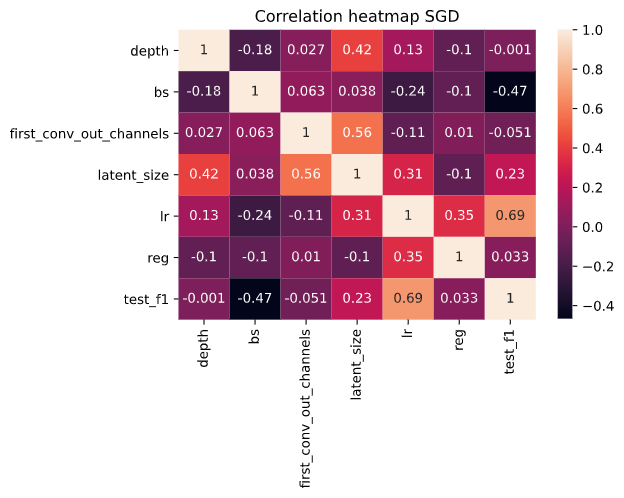
\includegraphics[width=.8\linewidth]{imagenes/06_Experimentacion/caeimages/caesgdcorr.png}  
  \caption{Correlación entre los hiperparámetros y \textit{test\_f1} para los resultados del optimizador \textit{SGD} (experimento CAE).}
  \label{fig:caesgdcorr}
\end{figure}

\subsection{Análisis resultados \textit{Convolutional Classifier}}

\begin{figure}[H]
\begin{subfigure}[b]{.5\textwidth}
  \centering
  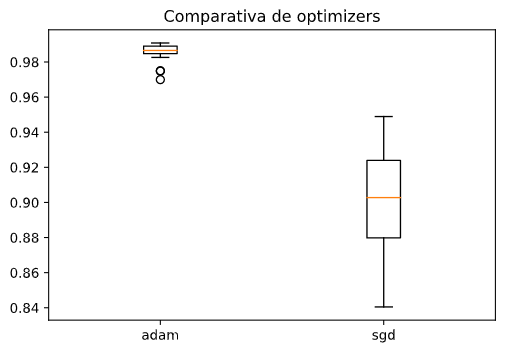
\includegraphics[width=.8\linewidth]{imagenes/06_Experimentacion/simplecnn/simplecnnboxplot.png}
  \caption{\textit{Optimizers boxplot}.}
  \label{fig:simplecnnoptimizers}
\end{subfigure}
\begin{subfigure}[b]{.5\textwidth}
  \centering
  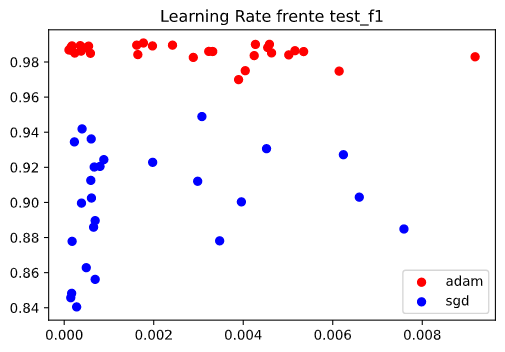
\includegraphics[width=.8\linewidth]{imagenes/06_Experimentacion/simplecnn/simplecnnlr.png}  
  \caption{\textit{Learning rate} frente \textit{$F_1$ score}.}
  \label{fig:simplecnnlr}
\end{subfigure}\\

\begin{subfigure}[b]{.5\textwidth}
  \centering
  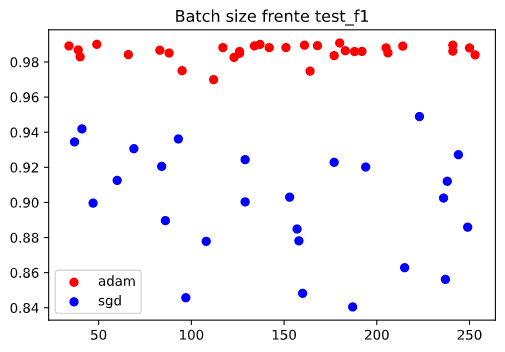
\includegraphics[width=.8\linewidth]{imagenes/06_Experimentacion/simplecnn/simplecnnbs.png}
  \caption{\textit{Batch Size} frente \textit{$F_1$ score}.}
  \label{fig:simplecnnreg}
\end{subfigure}

\caption{Plots para analizar del efecto de los hiperparámetros en los resultados del experimento Simple CNN.}
\label{fig:simplecnnanalysis}
\end{figure}

De los \textit{plots} de la Figura \ref{fig:simplecnnanalysis} podemos sacar las siguientes conclusiones:

\begin{itemize}
    \item De nuevo con \textit{Adam} se obtinen mejores resultados que con \textit{SGD}, pero esta vez la diferencia es mayor (esto se puede observar en la Figura \ref{fig:simplecnnoptimizers}).

    \item Con \textit{Adam} se obtienen buenos resultados independientemente del \textit{learning rate}. Sin embargo, con \textit{SGD} no hay mucha correlación entre el valor de este hiperparámetro y la métrica \textit{test\_f1} (esto se puede ver en la Figura \ref{fig:simplecnncorr}).
    
    \item Al igual que en el punto anterior, con \textit{Adam} también se obtienen buenos resultado independientemente del valor del \textit{batch size}. Con \textit{SGD} hay una correlación negativa baja entre este hiperparámetro y la métrica \textit{test\_f1} (ver Figura \ref{fig:simplecnncorr}).
\end{itemize}

\begin{figure}[H]
  \centering
  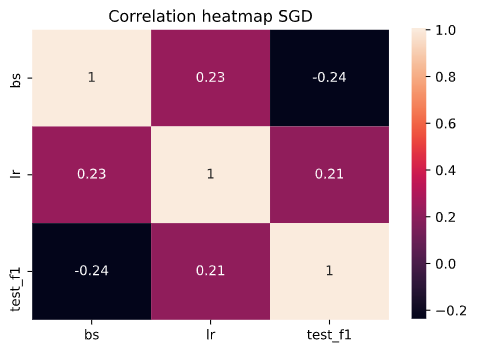
\includegraphics[width=.8\linewidth]{imagenes/06_Experimentacion/simplecnn/simplecnnsgdcorr.png}  
  \caption{Correlación entre los hiperparámetros y \textit{test\_f1} para los resultados del optimizador \textit{SGD} (experimento Simple CNN).}
  \label{fig:simplecnncorr}
\end{figure}

\subsection{Análisis resultados \textit{ResNet}}

\begin{figure}[H]
\begin{subfigure}[b]{.5\textwidth}
  \centering
  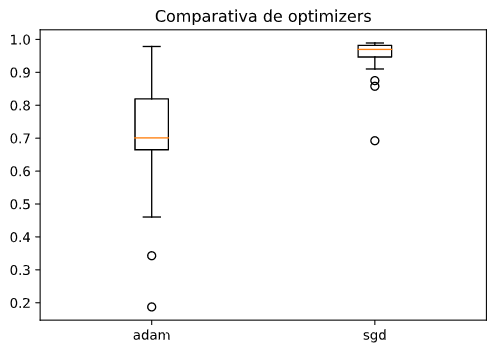
\includegraphics[width=.8\linewidth]{imagenes/06_Experimentacion/resnet/resnetboxplot.png}
  \caption{\textit{Optimizers boxplot}.}
  \label{fig:resnetoptimizers}
\end{subfigure}
\begin{subfigure}[b]{.5\textwidth}
  \centering
  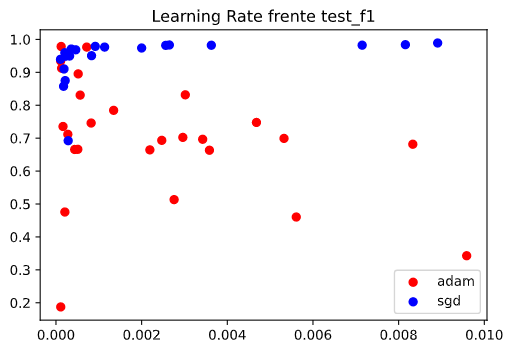
\includegraphics[width=.8\linewidth]{imagenes/06_Experimentacion/resnet/resnetlr.png}
  \caption{\textit{Learning rate} frente \textit{$F_1$ score}.}
  \label{fig:resnetlr}
\end{subfigure}\\

\begin{subfigure}[b]{.5\textwidth}
  \centering
  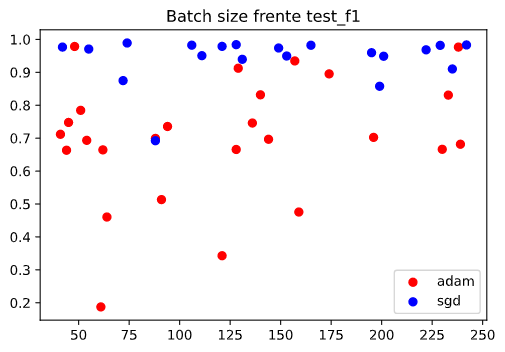
\includegraphics[width=.8\linewidth]{imagenes/06_Experimentacion/resnet/resnetbs.png}
  \caption{\textit{Batch Size} frente \textit{$F_1$ score}.}
  \label{fig:resnetbs}
\end{subfigure}
\begin{subfigure}[b]{.5\textwidth}
  \centering
  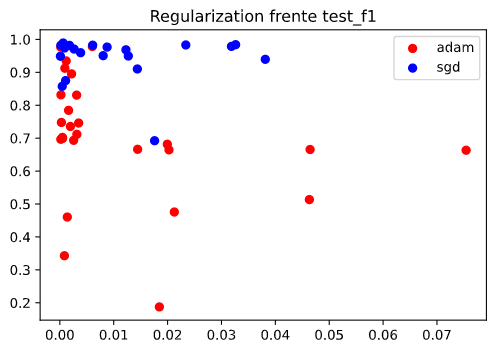
\includegraphics[width=.8\linewidth]{imagenes/06_Experimentacion/resnet/resnetreg.png}
  \caption{\textit{Regularization} frente \textit{$F_1$ score}.}
  \label{fig:resnetreg}
\end{subfigure}

\caption{Plots para analizar del efecto de los hiperparámetros en los resultados del experimento ResNet.}
\label{fig:resnetanalysis}
\end{figure}

De la Figura \ref{fig:resnetanalysis} podemos sacar las siguientes conclusiones:

\begin{itemize}
    \item Viendo la Figura \ref{fig:resnetoptimizers}, vemos que por primera vez \textit{SGD} saca mejores resultados que \textit{Adam} y por bastante (los resultados de \textit{SGD} están a la altura del Q4 de \textit{Adam} y la mediana es mucho más alta). De hecho, el mejor resultado para la métrica \textit{test\_f1} ha sido usando el optimizador \textit{SGD} (ver Tabla \ref{tab:results}).
    \item En la Figura \ref{fig:resnetlr} se puede observar que con el optimizador \textit{SGD} parece que se van obteniendo mejores resultados conforme se va aumentando el \textit{learning rate} aunque la correlación, que se puede ver en la Figura \ref{fig:resnetsgdcorr}, no es muy alta. En cambio, con \textit{Adam} parece que con un \textit{learning rate} alto va dando peores resultados, aunque la correlación (ver Figura \ref{fig:resnetadamcorr}) también es débil.
    \item Observando la Figura \ref{fig:resnetbs} parece no haber relación entre el \textit{Batch Size} y la métrica \textit{test\_f1}, de hecho la correlación es débil (ver Figura \ref{fig:resnetsgdcorr} y Figura \ref{fig:resnetadamcorr}).
    \item Viendo la Figura \ref{fig:resnetreg}, podemos confirmar que la regularización no tiene efecto notable en el resultado del optimizador \textit{SGD}. En el caso de \textit{Adam}, parece que el valor de regularización tampoco afecta demasiado al resultado.
\end{itemize}

\begin{figure}[H]
\begin{subfigure}[b]{.5\textwidth}
  \centering
  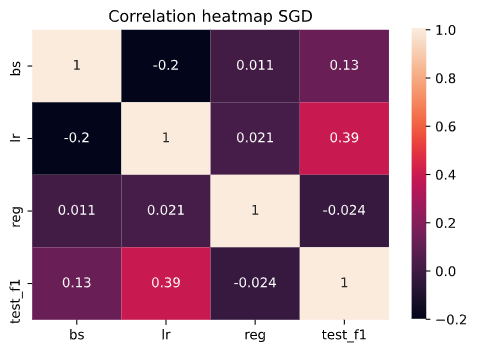
\includegraphics[width=.8\linewidth]{imagenes/06_Experimentacion/resnet/resnetsgdcorr.png}
  \caption{Correlación entre los hiperparámetros y \textit{test\_f1} para los resultados del optimizador \textit{SGD}.}
  \label{fig:resnetsgdcorr}
\end{subfigure}
\begin{subfigure}[b]{.5\textwidth}
  \centering
  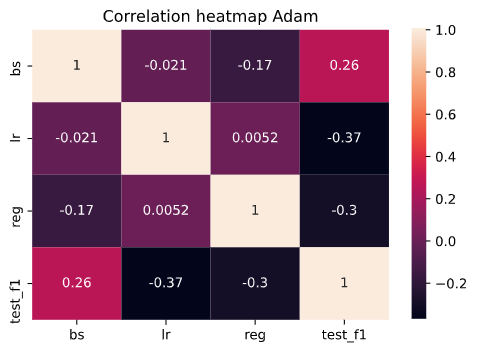
\includegraphics[width=.8\linewidth]{imagenes/06_Experimentacion/resnet/resnetadamcorr.png}
  \caption{Correlación entre los hiperparámetros y \textit{test\_f1} para los resultados del optimizador \textit{Adam}.}
  \label{fig:resnetadamcorr}
\end{subfigure}

\caption{Matrices de correlación entre los hiperparámetros y la métrica \textit{test\_f1} (experimento ResNet).}
\label{fig:resnetcorrelationmatrices}
\end{figure}

\subsection{Análisis de resultados \textit{Varitional Autoencoder}}

\begin{figure}[H]
\begin{subfigure}[b]{.5\textwidth}
  \centering
  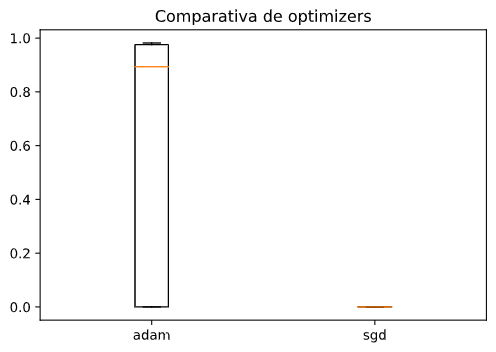
\includegraphics[width=.8\linewidth]{imagenes/06_Experimentacion/vae/vaeboxplot.png}
  \caption{\textit{Optimizers boxplot}.}
  \label{fig:vaeoptimizers}
\end{subfigure}
\begin{subfigure}[b]{.5\textwidth}
  \centering
  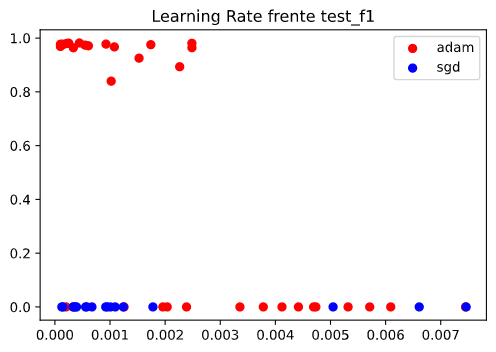
\includegraphics[width=.8\linewidth]{imagenes/06_Experimentacion/vae/vaelr.png}
  \caption{\textit{Learning rate} frente \textit{$F_1$ score}.}
  \label{fig:vaelr}
\end{subfigure}\\

\begin{subfigure}[b]{.5\textwidth}
  \centering
  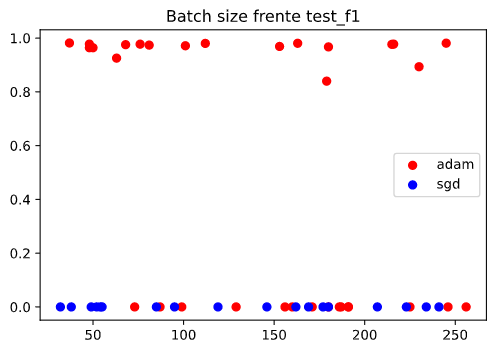
\includegraphics[width=.8\linewidth]{imagenes/06_Experimentacion/vae/vaebs.png}
  \caption{\textit{Batch Size} frente \textit{$F_1$ score}.}
  \label{fig:vaebs}
\end{subfigure}
\begin{subfigure}[b]{.5\textwidth}
  \centering
  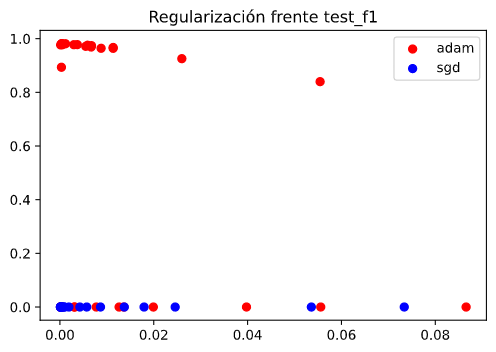
\includegraphics[width=.8\linewidth]{imagenes/06_Experimentacion/vae/vaereg.png}
  \caption{\textit{Regularization} frente \textit{$F_1$ score}.}
  \label{fig:vaereg}
\end{subfigure}

\caption{Plots para analizar del efecto de los hiperparámetros en los resultados del experimento VAE.}
\label{fig:vaeanalysis}
\end{figure}

De la Figura \ref{fig:resnetanalysis} podemos extraer las siguientes conclusiones:

\begin{itemize}
    \item Como se puede ver en la Figura \ref{fig:vaeoptimizers}, con \textit{SGD} no podemos entrenar un modelo que sea capaz de predecir, solo podemos usar \textit{Adam} para obtener unos resultados aceptables. Por tanto, en los siguientes puntos solo hablaré sobre los resultados obtenidos con este optimizador.
    \item Sobre el \textit{learning rate}, si es mayor que 0.003 es imposible obtener buenos resultados (como se puede ver en la Figura \ref{fig:vaelr}). Además, en la Figura \ref{fig:vaecorr} que hay una correlación negativa fuerte entre \textit{lr} y \textit{test\_f1}, confirmando mi afirmación.
    \item El \textit{Batch Size} no parece influir mucho en la métrica resultante, parece que al aumentar el valor es probable que de peor resultado como se puede ver en la Figura \ref{fig:vaebs} y en la Figura \ref{fig:vaecorr} se puede observer una correlación débil negativa.
    \item Viendo la Figura \ref{fig:vaereg} casi se puede afirmar que al aumentar el valor de la regularización, se va empeorando también el valor de la métrica \textit{test\_f1}.
\end{itemize}

\begin{figure}[H]
  \centering
  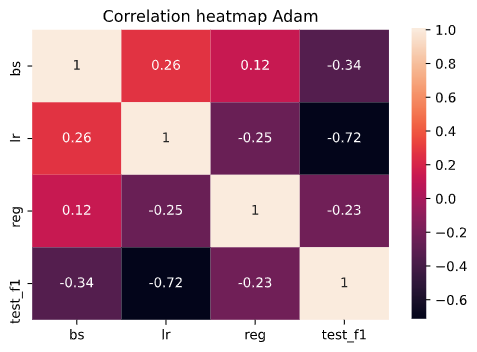
\includegraphics[width=.8\linewidth]{imagenes/06_Experimentacion/vae/vaeadamcorr.png} 
  \caption{Correlación entre los hiperparámetros y \textit{test\_f1} para los resultados del optimizador \textit{Adam} (experimento VAE).}
  \label{fig:vaecorr}
\end{figure}

\subsection{Análisis del uso de normalización}

Esta subsección ha sido añadida debido a un descuido que tuve (se me olvidó probar los resultados con los datos sin normalizar y normalizados para comparar resultados). En cuanto al análisis del efecto de la normalización, viendo los \textit{plots} de la Figura \ref{fig:normalization} podemos sacar las siguientes conclusiones:

\begin{itemize}
    \item Primeramente, en la Figura \ref{fig:caenorm} podemos ver que para el \textit{Convolutional Autoencoder} el uso de normalización empeora los resultados un poco para el caso del optimizador \textit{Adam} y bastante para el caso del optimizador \textit{SGD}.
    \item Para el caso de \textit{ResNet}, como se puede ver en la Figura \ref{fig:resnetnorm}, los resultados del \textit{SGD} mejoran un poco (el limite inferior de Q1 está más alto y el límite superior del Q4 está un poco más alto), pero se empeoran para \textit{Adam}.
    \item Para el caso de \textit{ConvClassifier} (ver Figura \ref{fig:simplecnnnorm}) y usando el optimizador \textit{SGD}, se obtienen mejores resultados sin regularización, pues la mediana está más alta y también el límite inferior de Q1 y el límite superior de Q4. Con el optimizador \textit{Adam}, parece que también se obtienen mejores resultados sin usar normalización, aunque la mediana esté más alta cuando se usa regularización, el límite superior de Q4 está más alto cuando no se usa regularización.
    \item Por último, con el modelo \textit{Varitional Autoencoder} (ver Figura \ref{fig:vaenorm}), los resultados con \textit{SGD} son claramente mejores cuando se usa normalización. En cuanto a \textit{Adam}, los resultados son mucho peores cuando se usa normalización.
\end{itemize}

\begin{figure}[H]
\begin{subfigure}{.5\textwidth}
  \centering
  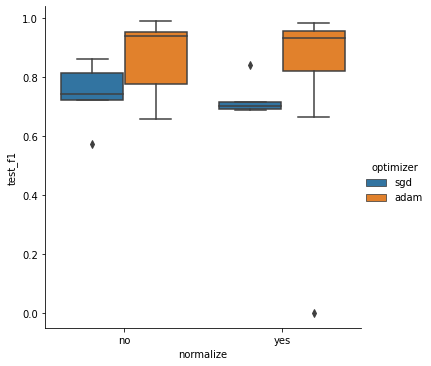
\includegraphics[width=.8\linewidth]{imagenes/06_Experimentacion/normalization/caenorm.png}  
  \caption{\textit{Plot} para análisis del efecto de la normalización en el modelo CAE.}
  \label{fig:caenorm}
\end{subfigure}
\begin{subfigure}{.5\textwidth}
  \centering
  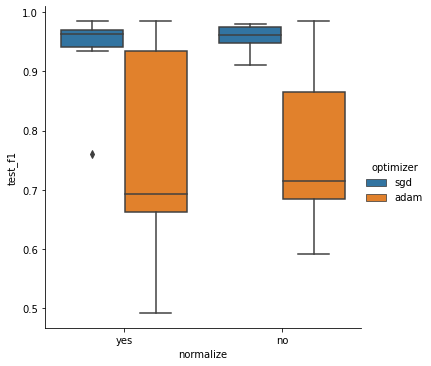
\includegraphics[width=.8\linewidth]{imagenes/06_Experimentacion/normalization/resnetnorm.png}  
  \caption{\textit{Plot} para análisis del efecto de la normalización en el modelo ResNet.}
  \label{fig:resnetnorm}
\end{subfigure}

\newline

\begin{subfigure}{.5\textwidth}
  \centering
  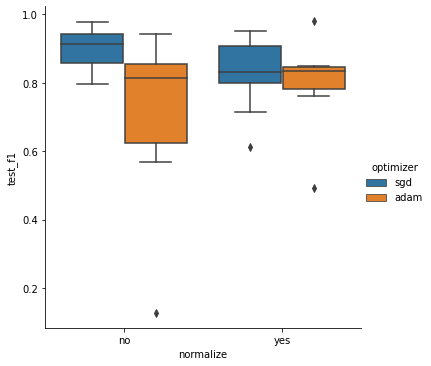
\includegraphics[width=.8\linewidth]{imagenes/06_Experimentacion/normalization/simplecnnnorm.png}  
  \caption{\textit{Plot} para análisis del efecto de la normalización en el modelo SimpleCNN.}
  \label{fig:simplecnnnorm}
\end{subfigure}
\begin{subfigure}{.5\textwidth}
  \centering
  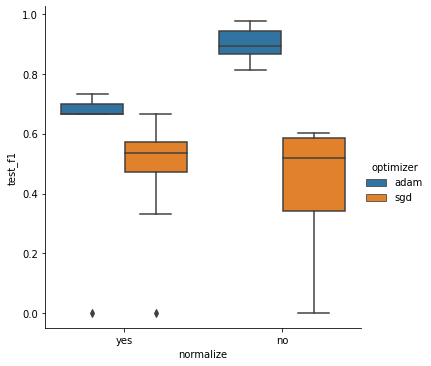
\includegraphics[width=.8\linewidth]{imagenes/06_Experimentacion/normalization/vaenorm.png}  
  \caption{\textit{Plot} para análisis del efecto de la normalización en el modelo VAE.}
  \label{fig:vaenorm}
\end{subfigure}
\caption{\textit{Plots} para análisis del efecto de la normalización.}
\label{fig:normalization}
\end{figure}

%
\chapter{Despliegue de modelos de Machine Learning}\label{chap:deploy}

En los anteriores capítulos se ha explicado el flujo de trabajo seguido y levantado la infraestructura necesaria para ello, además de haber entrenado bastantes modelos con buenos resultados en lo que a métricas se refiere. Pero, ¿se ha resultado algún problema? La respuesta es no. Falta el paso más importante que desplegar nuestros modelos en la infraestructura destino o dispositivo destino.\\

En este capítulo se va a comentar cómo sería el despliegue de los modelos que están almacenados en \textit{mlflow} para levantar un microservicio o hacer funcionar un dispositivo de \textit{Edge Computing} usando un despliegue continuo. Me gustaría recalcar que nada de lo explicado en este Capítulo se ha llevado a práctica por falta de tiempo, pero no me podía olvidar de explicar lo más importante del \textit{workflow}.\\

\section{Despliegue en un microservicio}

Desplegar un microservicio es muy sencillo hoy en día gracias a servicios \textit{serverless} como \textit{AWS Lambda}, a herramientas de provisionamiento como \textit{Terraform} o de orquestación como \textit{Ansible} \cite{ansible} (para uasr un IaaS como podría ser \textit{AWS EC2}) o a servicios PaaS como \textit{Heroku}. En este último podemos desplegar aplicaciones contenedorizadas o no y contiene otros servicios de bases de datos \textit{SQL}, \textit{logging}, monitorización, etc. Por tanto, haré hincapié en este plataforma debido a que puede satisfacer más casos de uso de forma muy simple.\\

Para realizar el despliegue sería tan fácil como instalar la CLI de \textit{Heroku} (o usando herramientas de orquestación como \textit{Ansible} en el caso de IaaS) en el contenedor usado para ejecutar el \textit{pipeline} de Integración Continua y notificar en un \textit{stage} que se ejecuta al final si todos los anteriores han sido exitosos a \textit{Heroku} para volver a desplegar el contenedor o servicio actualizado.\\

Pero el problema es, ¿Cómo podemos obtener los modelos almacenados en \textit{mlflow}? Esto es bastante sencillo puesto que tiene una API para hacer \textit{queries} \cite{mlflowtrackingapi} y obtener todos los artefactos generados por un experimento, como se puede ver a continuación:\\

\begin{lstlisting}[language=Python, caption={Script de Python para obtener el modelo que maximiza la métrica \textit{test\_f1}}, captionpos=b, label=lst:getmodel]
import os
import sys
from mlflow.tracking import MlflowClient
from mlflow.entities import ViewType

tracking_uri = os.getenv("MLFLOW_TRACKING_URI")

if tracking_uri is None:
    sys.exit("MLFLOW_TRACKING_URI environment variable not defined.")

# Conexion al servidor mlflow
client = MlflowClient(tracking_uri)

# Obtener todos los experimentos
experiments = client.list_experiments()
experiments_ids = []

# Obtener todos los IDs de los experimentos
for experiment in experiments:
    experiments_ids.append(experiment.experiment_id)

# Obtener la run que maximiza la metrica test_f1
best_run = client.search_runs(
    experiments_ids,
    run_view_type=ViewType.ACTIVE_ONLY,
    order_by=["metrics.test_f1 DESC"],
    max_results=1,
)

if len(best_run) == 0:
    sys.exit("No runs found or invalid MLFLOW_TRACKING_URI.")

# Descargar el modelo almacenado en S3
best_run = best_run[0]
client.download_artifacts(
    best_run.info.run_id, path="model.pth", dst_path="artifacts"
)
\end{lstlisting}

El script anterior se encarga de recuperar el modelo que maximice la métrica \textit{test\_f1}, esto nos puede ser últil de cada a desplegarlo (incluso se podría implementar como una tarea de \textit{invoke}). Para ejecutar ese script harían falta tres variables de entorno:

\begin{itemize}
    \item \textbf{MLFLOW\_TRACKING\_URI.} Dirección de nuestro servidor de \textit{mlflow}.
    \item \textbf{AWS\_ACCESS\_KEY\_ID.} Si los modelos se guardan en \textit{AWS S3}, esta variable de entorno es necesaria para poder acceder al \textit{bucket}.
    \item \textbf{AWS\_SECRET\_ACCESS\_KEY.} Si los modelos se guardan en \textit{AWS S3}, esta variable de entorno es necesaria para poder acceder al \textit{bucket} al igual que la anterior.
\end{itemize}

\begin{lstlisting}[language=docker, caption={Dockerfile para desplegar nuestro microservicio en Heroku o en cualquier máquina}, captionpos=b]
FROM python:3.8-slim AS base

RUN groupadd python \
    && useradd -r --home-dir /home/python --shell /bin/bash -g python python \
    && mkdir /home/python \
    && chown -R python:python /home/python

USER python

ENV PATH=${PATH}:/home/python/.local/bin

WORKDIR /home/python

RUN pip install poetry

# Copiamos los ficheros importantes para el despliegue
COPY poetry.lock pyproject.toml tasks.py app/ src/ ./

# Instalamos dependencias
RUN poetry export -f requirements.txt --without-hashes | pip install -r /dev/stdin

ENTRYPOINT invoke get_model && invoke start

\end{lstlisting}

En el \path{Dockerfile} anterior se definen las órdenes necesarias para poner en producción el microservicio (siguiendo las buenas prácticas mencionadas en la Subsección \ref{subsec:dockerpractices}). Al ejecutar el contenedor creado, se llama a la \textit{task} denominada \textit{get\_model} (hace lo mismo que el script contenido en el Listing \ref{lst:getmodel}) y luego a \textit{start} (inicia el microservicio que carga el modelo para poder funcionar). Es importante definir también las variables de entorno en la máquina donde se realice el despliegue\footnote{Con \textit{Terraform} se puede editar el fichero \path{.bashrc} para establecerlas en tiempo de aprovisionamiento y en \textit{Heroku} se puede hacer fácilmente desde la interfaz \textit{web} o desde la CLI}.\\

Por último, nos queda definir el despliegue en nuestra plataforma de CI/CD. En esta ocasión, tal y como señalé en la Subsección \ref{subsec:cicdplatforms}, estoy usando \textit{Jenkins} pero puede ser cualquier otra. Para configurar el despliegue continuo, bastaría con añadir un \textit{stage} o un paso al final de todo y que se ejecute si los demás (\textit{tests} y \textit{linters}) han sido exitosos. En mi caso (ver Figura \ref{fig:jenkinspipeline}) añadiría el \textit{stage} de despliegue después del \textit{stage} paralelo que ejecuta los \textit{linters} y los \textit{tests}.\\

\begin{figure}[H]
  \centering
  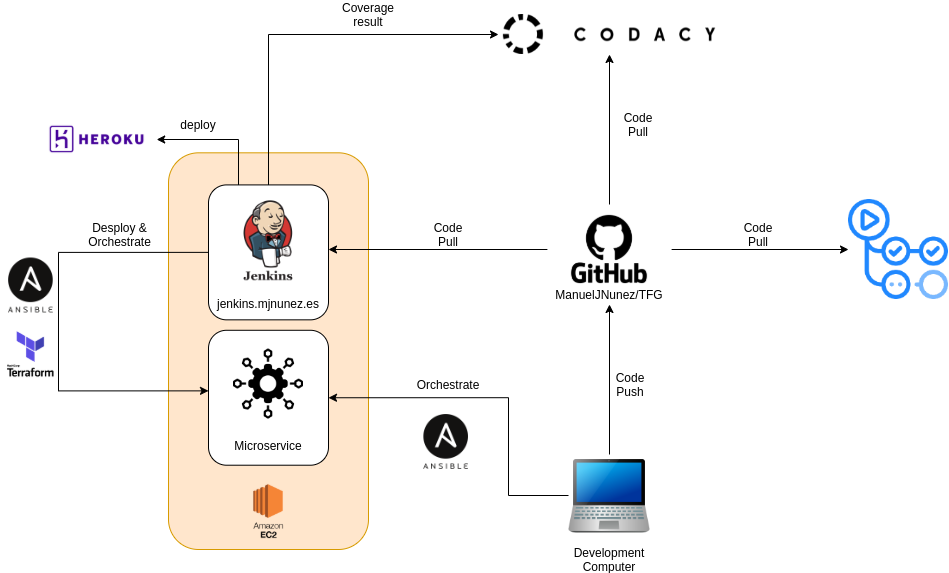
\includegraphics[width=1.\linewidth]{imagenes/07_Despliegue/TFGdiagrams-CICD.png} 
  \caption{Diagrama de cómo sería la infraestructura de \textit{testing} y de despliegue (usando \textit{Heroku} o \textit{AWS EC2}).}
  \label{fig:cicd}
\end{figure}

En la Figura \ref{fig:cicd} se muestran dos herramientas bastante importantes anteriormente nombradas, \textit{Ansible} y \textit{Terraform}. \textit{Ansible} no serviría por ejemplo para orquestar nuestra máquina o máquinas y cada vez que se producen cambios actualizar el código desplegado y volver a arrancar la aplicación. \textit{Terraform} nos valdría para controlar la infraestructura de nuestra aplicación desplegada. La infraestructura puede ser además orquestada desde la máquina de desarrollo.\\

En esta sección se ha puesto de ejemplo \textit{AWS EC2} pero se puede usar cualquier otro servicio de IaaS como \textit{GCP Compute Engine} y también se ha hablado de \textit{Heroku} pero se puede usar cualquier otro servicio de PaaS como el de \textit{Digital Ocean}. El único límite es la imaginación del desarrollador.\\

\begin{figure}[H]
  \centering
  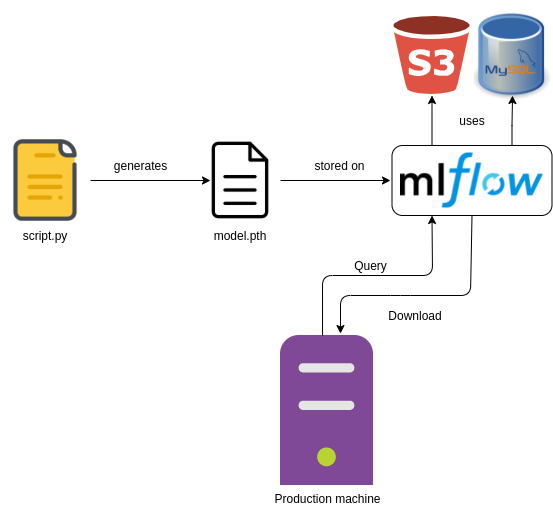
\includegraphics[width=.8\linewidth]{imagenes/07_Despliegue/ModelLifecycle.png} 
  \caption{Ciclo de vida de los modelos entrenados.}
  \label{fig:modellifecycle}
\end{figure}

En la anterior Figura \ref{fig:modellifecycle} se puede observar el ciclo de vida de un modelo desde que se genera, se serializa en un fichero que es almacenado a través de \textit{mlflow} en \textit{S3} y sus métricas e hiperparámetros son almacenados en la base de datos. La máquina en la que se mandan los modelos a producción realiza \textit{queries} (usando por ejemplo el script del Listing \ref{lst:getmodel}) para descargar el modelo que maximice la métrica objetivo.

\section{Despliegue en el contexto del \textit{Edge Computing}}

En este contexto, el diseño más habitual es el del \textit{publisher}/\textit{subscriber}. Es decir, tenemos dispositivos empotrados con sensores que publican datos y un computador central (o varios) que se subscribe a ellos a través de una red. Para la implementación de este sistema podemos usar librerías como \textit{ZeroMQ}. También podemos contar con \textit{RTI Connector} \cite{rticonnector} (una versión simple de \textit{RTI Connext DDS} para \textit{Python} y \textit{JavaScript}) que al igual que ZeroMQ no necesita de ningún \textit{broker} y podrían permitir que el diseño del sistema sea más escalable en comparación con \textit{MQTT}.\\

Como se puede ver a simple vista, este tipo de sistemas es más complejo que uno de microservicios, pues tenemos más de un dispositivo con distintas responsabilidades (unos publican por ejemplo la temperatura, otros el estado de algún objeto, otros leen los datos para procesarlos, etc). Otra dificultad que podría haber en estos dispositivos es que no tienen por qué estar 24h activos.\\

Este sería el tipo de despliegue más interesante en el contexto del problema que se pretende resolver con el conjunto de datos con el que he sido provisto (ver Sección \ref{sec:problemdesc}). Generalmente, interesa que una red de sensores sea escalable, por lo que sería interesante buscar una solución escalable que nos permita añadir nuevos nodos sin problema.\\

En este escenario, una solución basada en orquestación de contenedores (como \textit{Kubernetes} \cite{kubernetes} o \textit{Nomad} \cite{nomad}) o de orquestación de sistemas (usando \textit{Ansible} por ejemplo) sería totalmente obligatoria para controlar todo el sistema y su funcionamiento. Y no quedaría ahí, también sería esencial monitorizar todos los sistemas (se puede usar un \textit{software} como por ejemplo \textit{Grafana} \cite{grafana}, muy popular por su interfaz o \textit{Zabbix} \cite{zabbix}) y por supuesto, recoger los logs de las aplicaciones para poder ver el estado de las aplicaciones desplegadas (para ello existen herramientas online como por ejemplo \textit{logdna} \cite{logdna} o \textit{Papertrail} \cite{papertrail}). Estas herramientas no solo son útiles en el contexto de \textit{Edge Computing}, también sería interesante su uso en el despliegue de un microservicio.\\

Para monitorizar este tipo de sistemas, se puede hacer a través de la creación de un \textit{topic} denominado \textit{health} (para el caso de \textit{RTI Connector} o un tipo de mensaje especial para el caso de \textit{ZeroMQ}) a través del cual la aplicación de monitorización pregunta a todos los nodos si están funcionando correctamente. Si alguno no está funcionando no respondería y la aplicación de monitorización avisaría del estado. En el contexto de un microservicio, esto se haría mediante el uso de un \textit{health endpoint} (que devuelve 200 si todo ha ido bien). Mediante el uso de los sistemas de \textit{logging} distribuido anteriormente nombrado podemos además acceder a información sobre los mensajes de información, avisos o excepciones de las aplicaciones. Por último, recalcar que también sería necesaria la monitorización del uso de CPU, memoria, red, etc para evitar posibles saturaciones del sistema.

%
\chapter{Conclusiones y Trabajos Futuros}

\section{Conclusiones}

En este trabajo se ha intentado hacer una guía lo más completa posible del campo del \textit{Machine Learning} desde la perspectiva de la Ingeniería. En los capítulos anteriores se ha llegado a una solución usando las prácticas de \textit{DevOps} en el contexto del \textit{Machine Learning}, lo cual recibe el nombre de \textit{MLOps}. Sobre esto último no hay muchos trabajos publicados en internet.\\

La solución propuesta hace uso de contenedores y de software libre de tal forma que los experimentos y la infraestructura virtual usada en este trabajo son reproducibles por cualquier persona o entidad (usando la \textit{cloud} o incluso su propia infraestructura). Para poder reproducir lo anterior mencionado, se ha dejado una guía en el fichero \path{README.md} del repositorio de \textit{GitHub}.\\

Por otro lado, se ha conseguido unos resultados muy buenos en el problema que se pretendía resolver en este trabajo, llegando a un valor de 0.99 para la métrica $F_1$ en el conjunto de pruebas y además pudiendo analizar cuáles son los hiperparámetros que mayor efecto tienen sobre la métrica que mide la capacidad predictiva del modelo entrenado.\\

Gracias al uso de la herramienta \textit{mlflow} se ha podido llevar un \textit{tracking} de los experimentos, es decir, se ha podido guardar los hiperparámetros con los que se han entrenado los modelos y las métricas. Además, ha permitido almacenar automáticamente el modelo entrenado para su posterior descarga y despliegue en otra máquina y algunos \textit{plots} (como la matriz de confusión) para su posterior análisis. Y por último, mencionar la gran utilidad del framework \textit{SnapperML}, con el cual he podido definir los experimentos en ficheros con formato \textit{YAML} para poder ejecutar los experimentos fácilmente y guardar los resultados y artefactos en \textit{mlflow}.

\section{Trabajos Futuros}

Este trabajo constituye solo la primera parte de mi estudio sobre las técnicas de \textit{MLOps}, ya tengo listo el \textit{workflow} para entrenar modelos y he ideado como sería el despliegue del modelo en un microservicio y en el contexto del \textit{Edge Computing} (ver Capítulo \ref{chap:deploy}). Claramente, los siguientes pasos de este trabajo serían aprender sobre herramientas de orquestación para hacer pruebas de concepto de cómo sería el despliegue en el observatorio (o cualquier otro dentro del contexto del \textit{Edge Computing}), además de probar y añadir la infraestructura necesaria para monitorización y \textit{logging}.\\

Además, se podría adaptar el \textit{workflow} actual a \textit{kubernetes} para hacer que el despliegue de \textit{mlflow} y de los servicios que usa \textit{SnapperML} sea realizado con una única orden y por tanto de forma más sencilla. Por último, recalcar que también sería interesante implementar \textit{tests} de infraestructura para comprobar que la infraestructura levantada funciona tal y como está planificado que lo haga.\\

%

% \nocite{*}
\bibliography{bibliography/bibliography}%\addcontentsline{toc}{chapter}{Bibliografía}
\bibliographystyle{plain}
%
%\appendix
%\input{apendices/manual_usuario/manual_usuario}
%\input{glosario/entradas_glosario}
% \addcontentsline{toc}{chapter}{Glosario}
% \printglossary
%\chapter*{}
%\thispagestyle{empty}

\end{document}
